%\documentclass{report}
\documentclass[a4paper,12pt]{article}
\usepackage[utf8]{inputenc}
\usepackage[italian]{babel}
\usepackage{graphicx}
\usepackage{booktabs}
\usepackage{geometry}
\usepackage{lipsum}
\usepackage{amsmath}
\usepackage{amsfonts}
\usepackage{amsthm}
\usepackage{wrapfig}
\usepackage[dvipsnames]{xcolor}
\usepackage{xurl}
\usepackage{multirow}
\usepackage[hidelinks]{hyperref}
\usepackage{xcolor}
\definecolor{light-gray}{gray}{0.95}
\newcommand{\code}[1]{\colorbox{light-gray}{\texttt{#1}}}
\newgeometry{
    top=0.7 in,
    bottom=0.7in,
    outer=0.7in,
    inner=0.7in,
}
\usepackage{todonotes}
\usepackage[backend=biber]{biblatex}
\addbibresource{bibliography.bib}

\title{Approcci 2D e 3D per l'analisi e la modellazione digitale di capi d'abbigliamento\\
{\Large Università di Verona}}
\author{Rosa Russo}
%\date{Giugno 2022}

\begin{document}
\maketitle

\todo[inline]{
- Motivare scelta articoli \\
- Aggiungere DeePSD
}
%\tableofcontents
%\chapter{Fase di studio e analisi del lavoro esistente}
\section{Fase di studio e analisi del lavoro esistente}
\subsection{Introduzione}

In questo paragrafo viene spiegato brevemente il percorso di analisi del lavoro esistente riguardo la modellazione virtuale di vestiti su mesh tre-dimensionali.

\paragraph{Mesh}
Una mesh poligonale è la partizione di una superficie continua in celle poligonali, come triangoli, quadrilateri, ecc.
Più formalmente, una mesh \( M \) può essere definita come una \emph{tupla} \( (V, K) \), dove 
\[
V = \{ \mathbf{v}_i \in \mathbb{R}^3 \mid i = 1, \ldots, N_v \}
\]
è l'insieme dei vertici del modello (punti in \( \mathbb{R}^3 \)) e \( K \) contiene l'\emph{adjacency information}, ovvero come i vertici sono connessi per formare gli spigoli e le facce della mesh.

\paragraph{Review}
Inizialmente sono stati studiati articoli che riguardano l’estrazione di mesh del corpo umano partendo da immagini e video, ma per seguire questa strada c’è bisogno prima di stimare la forma del corpo del soggetto in esame e poi procedere all’estrazione delle mesh dei singoli vestiti separate da quella del corpo stesso. Per questa ragione si è passati poi alla ricerca di dataset contenenti scansioni 3D e articoli di lavori correlati riguardanti la stratificazione di mesh inerenti a corpo umano nudo ed indumenti indossati.

Tra i lavori ritenuti interessanti troviamo un self-supervised framework (\href{https://openaccess.thecvf.com/content/ICCV2021/papers/Sanyal_Learning_Realistic_Human_Reposing_Using_Cyclic_Self-Supervision_With_3D_Shape_ICCV_2021_paper.pdf}{SPICE}) \cite{sanyal2021learning} che, partendo dall’immagine di una persona, è in grado di generare una nuova immagine di tale soggetto in una posa target, raggiungendo performance dello stato dell’arte sul DeepFashion dataset, con prestazioni migliori rispetto a metodi non supervisionati e simili allo stato dell’arte di metodi supervisionati. SPICE, inoltre, genera video partendo da una singola immagine data in input ed una sequenza di pose, nonostante sia stato addestrato solo su immagini statiche.

\medskip

\subsection{Approcci 2D}

Volendo partire da immagini 2D per predire il volume del corpo umano svestito e la mesh dei vestiti indossati, sono stati analizzati i seguenti articoli:

\begin{itemize}
\item End-to-end Recovery of Human Shape and Pose,
\item Moulding Humans,
\item BodyNet,
\item Parsing clothing in fashion photograph,
\item Multi-garment Net.

\end{itemize}


\subsubsection{End-to-end Recovery of Human Shape and Pose}

In “End-to-end Recovery of Human Shape and Pose” \cite{kanazawa2018end} viene fatta una Human Mesh Recovery (HMR), viene ricostruita cioè una mesh 3D di un corpo umano, partendo dalle immagini RGB del dataset Human3.6M.
Da una GAN vengono generati parametri relativi a posa, shape e camera.
Questo sembrerebbe estrarre meglio il corpo senza vestiti rispetto a BodyNet e Moulding humans, ma non è sempre assicurato che la forma corrisponda alla realtà (ad esempio, per quanto riguarda foto di donne incinta, nella costruzione della forma 3D viene eliminata la pancia perché confusa con gli abiti). Questo perché la rete si occupa principalmente di generare una shape che sembri reale, piuttosto che ottenerne una corrispondente al corpo originale ritratto in foto.
Dunque necessiterebbe di migliorie quali l’aggiunta di tipi di forme del corpo non previste nel lavoro originale.
Il dataset Human3.6M, mette a disposizione 3.6 milioni di immagini di persone e le corrispondenti pose e mesh, acquisite mediante quattro camere digitali. I dati sono organizzati in quindici movimenti di training, tra i quali camminare con vari tipi di asimmetrie (per esempio, camminare con una mano nella tasca, o con una borsa sulla spalla), pose di persone in attesa, sedute o sdraiate, ecc. Tali movimenti sono stati eseguiti da undici attori professionisti, sei uomini e cinque donne, scelti per coprire un indice di massa corporea (BMI) da 17 a 29, in modo da fornire una moderata variabilità per quanto riguarda la forma del corpo e i diversi movimenti.

\newpage

\subsubsection{Moulding Humans}

“Moulding Humans” (2019 - \url{https://openaccess.thecvf.com/content_ICCV_2019/papers/Gabeur_Moulding_Humans_Non-Parametric_3D_Human_Shape_Estimation_From_Single_Images_ICCV_2019_paper.pdf}) usa immagini 2D e, tramite una GAN genera delle mappe di profondità che sono usate per ricostruire la forma della persona.
Stima le profondità dalla foto senza fare troppa distinzione tra clothed e non clothed, a differenza del HMR.


\subsubsection{BodyNet}
La rete neurale proposta, BodyNet (\url{https://arxiv.org/abs/1804.04875}), è una rete neurale in grado di produrre una stima della forma del corpo volumetrico, prendendo in input una singola immagine. Si tratta di una rete addestrabile end-to-end che beneficia di (i) una loss volumetrica 3D, (ii) una loss di riproiezione multi-view e (iii) supervisione intermedia della posa 2D, della segmentazione delle parti del corpo 2D e della posa 3D. Per la evaluation del metodo, viene adattato il modello SMPL all’output della rete BodyNet che prende in ingresso i dataset SURREAL e Unite the People. Tale rete è composta, dunque, da quattro moduli: (i) un modulo per l’estrazione della posa 2D, (ii) un modulo per estrarre una possibile segmentazione 2D, dopodichè (iii) i due moduli precedenti vengono combinati insieme all'immagine originale, permettendo di ottenere la posa 3D, e, infine, (iv) usando i 4 ingressi descritti precedentemente si ottiene in output la forma volumetrica, che viene usata come riferimento per ottimizzare il modello SMPL (che ottiene la unclothed shape).

\subsubsection{Parsing clothing in fashion photograph}
Nonostante l’abbigliamento determini gran parte della shape di una persona, ci sono stati relativamente pochi tentativi di riconoscimento computazionale dei capi di abbigliamento: ci si è focalizzati principalmente sull’identificazione delle parti del corpo, divise in superiore ed inferiore, per poi rappresentare l’abbigliamento come una deformazione del contorno del corpo sottostante. Di recente sono stati fatti dei tentativi per considerare i capi di abbigliamento come attributi semantici di una persona, ma solo per quanto riguarda un numero limitato di indumenti (come t-shirt, jeans, pantaloncini, ecc).
A differenza di tali approcci, in “Parsing clothing in fashion photograph” si cercano di stimare in maniera precisa le aree della superficie relative ad un’ampia lista di possibili capi indossati da un soggetto ( come scarpe, cappello, cintura, calzini, ecc).

\begin{figure}[ht!]
  \centering
  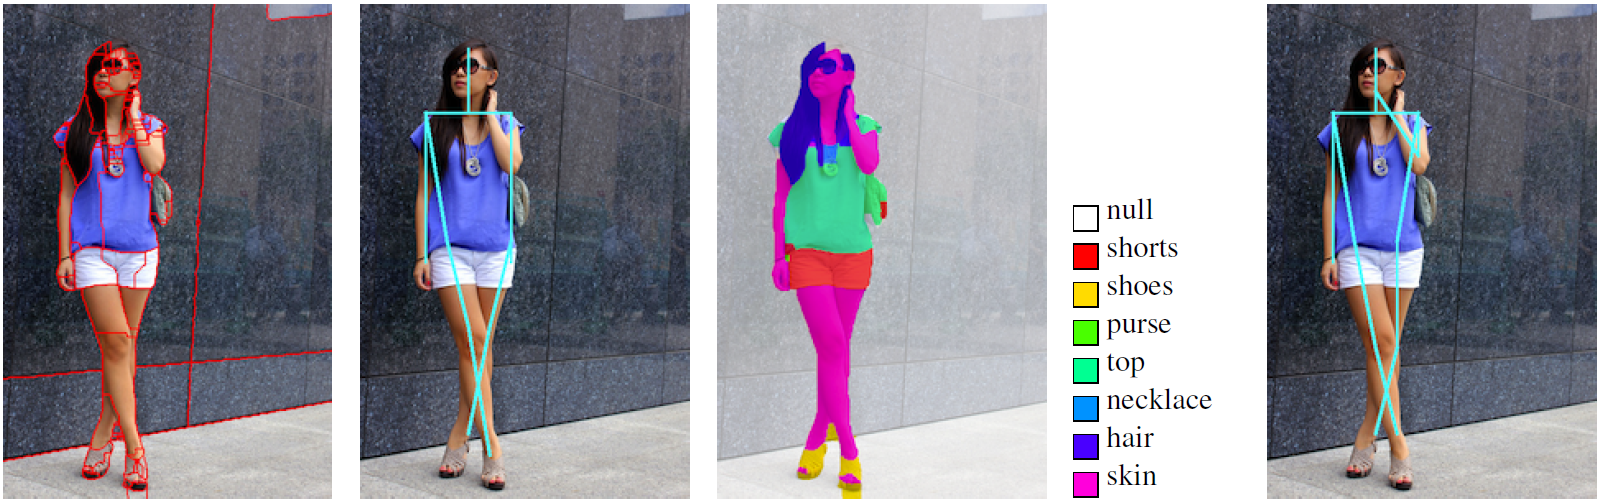
\includegraphics[scale=0.4]{Images/IntroductionPic/parsingclothing.png}
  \caption{(a) Superpixels (b) Stima della posa (c) Segmentazione dei capi di abbigliamento (d) Stima della posa finale }
  \label{fig:SMPL2}
\end{figure}
Per tale analisi, viene utilizzato un dataset che comprende 158’235 foto, con relativa descrizione, stile ed occasione per la quale l’outfit è stato indossato, ed un modello di riconoscimento che permette la segmentazione dei singoli capi di abbigliamento. Per semplificare tale processo, si assume che ogni capo di abbigliamento corrisponde ad una particolare area della superficie del corpo. In questo studio, la posa è fondamentale, in quanto può causare occlusioni importanti e di conseguenza complicare il riconoscimento degli abiti, per tale ragione viene effettuata anche una stima della posa a partire dall’immagine.

\medskip

\subsubsection{Multi-Garment Net}

In “Multi-Garment Net: Learning to Dress 3D People from Images” (\url{https://arxiv.org/pdf/1908.06903.pdf}) viene introdotta la rete multi-indumento (MGM, Multy-Garment Network), ovvero il primo modello in grado di posizionare dei layers esterni di vestiti (con mesh esclusive) direttamente sopra all’immagine data in input.
Come si può vedere nella figura sottostante, questa nuova rappresentazione permette il pieno controllo sulla forma del corpo, sulla struttura e geometria dell’abbigliamento e apre le porte ad una vasta gamma di applicazioni VR/AR, intrattenimento, cinematografiche e virtual try-on.

\begin{figure}[ht!]
  \centering
  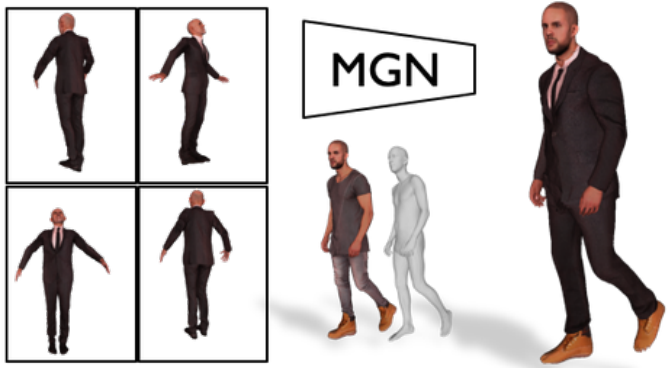
\includegraphics[scale=0.7]{Images/SizerPic/MultyGarmetNet.png}
  \caption{Da sinistra a destra: immagini dal soggetto sorgente, corpo dal
soggetto target, target vestito con indumenti originali. Da uno o
più immagini, MGN può ricostruire la forma del corpo e ciascuna di esse
i capi separatamente. Possiamo trasferire i capi previsti a
un corpo nuovo che include geometria e texture.}
    \label{fig:MultyGarmetNet}
\end{figure}

\newpage
Per raggiungere questo livello di controllo, MGM affronta due sfide principali:

\begin{enumerate}
\item apprendimento di un modello per ogni abito da scansioni tridimensionali di persone vestite
\item imparare a ricostruire tali modelli dalle immagini stesse
\end{enumerate}

\medskip

Per fare ciò, viene definito un insieme discreto di templates di abbigliamento (in base alle varie categorie: maglie lunghe/corte, pantaloni lunghi/corti e cappotti) e viene registrato, per ogni categoria, un singolo template per ciascuna delle istanze delle scansioni che vengono automaticamente segmentate in parti di vestito e pelle.
Poiché la geometria dell'indumento varia in modo significativo all'interno di una categoria (ad es. forme diverse, lunghezze delle maniche), per prima cosa viene ridotto al minimo la distanza tra il modello ed i bordi della scansione, cercando di preservare il laplaciano della superficie del modello.
In questo modo viene compilato un guardaroba digitale di veri capi 3D indossabili dalle persone (come mostrato sotto in Figura).

\medskip

\begin{figure}[ht!]
  \centering
  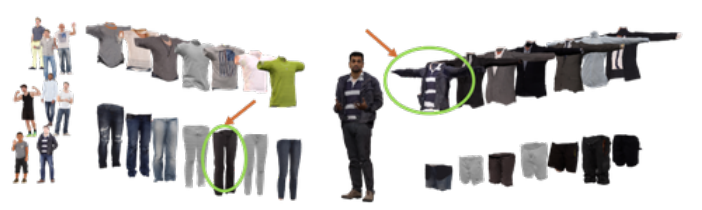
\includegraphics[scale=0.6]{Images/SizerPic/Sizer3.png}
  \caption{Viene utilizzato l'approccio di registrazione multi-mesh proposto per registrare i capi presenti nelle scansioni (a sinistra) su
modelli di indumenti fissi. Questo permette di costruire un guardaroba digitale e vestire soggetti arbitrari (al centro) selezionando i capi (segnati)
dall'armadio.}
    \label{fig:Sizer3}
\end{figure}

\medskip

A partire da tali registrazioni, viene introdotto un modello PCA basato sui vertici degli abiti.
Siccome gli indumenti sono associati (naturalmente) al sottostante modello SMPL, è possibile usarli su diverse morfologie del corpo e riposizionarli usando SMPL.

\medskip

Dal guardaroba digitale, MGM è addestrato a prevedere, data 
\begin{itemize}
\item una o più immagini della persona
\item posa del corpo
\item parametri della forma corporea
\end{itemize}

\medskip

I coefficienti PCA di ciascuno dei capi oltre che ad un “campo di variazione” sopra al modello PCA che codifica i dettagli dell’abbigliamento.
Al momento del test, vengono perfezionate queste stime bottom-up
con un nuovo obiettivo top-down che costringe gli indumenti e la pelle proiettati ad analizzare la segmentazione semantica dell'input.

\medskip

\begin{figure}[ht!]
  \centering
  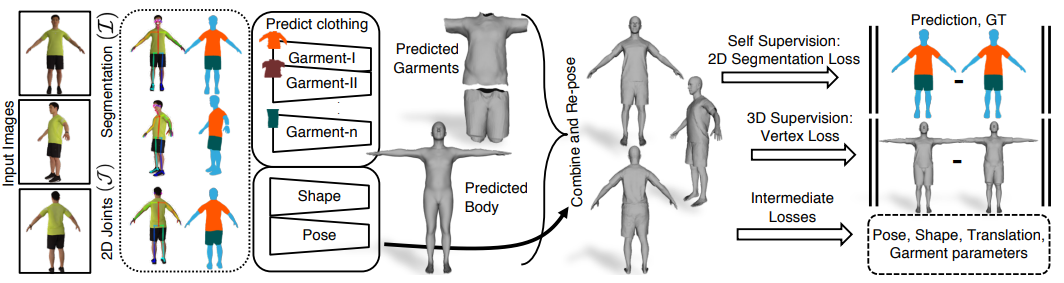
\includegraphics[scale=0.5]{Images/SizerPic/Sizer4.png}
  \caption{Dato un piccolo numero di frame RGB (attualmente 8), vengono pre-calcolate immagini segmentate semanticamente
$(I)$ e Giunti $2D (J)$. Il Multi-Garment Network (MGN), prende ${I,J}$ come input e deduce gli indumenti separabili e il sottostante
forma umana in una posa canonica. Queste previsioni vengono riposte usando le previsioni di posa per fotogramma. Viene fornito la  MGN con una combinazione di Supervisione 2D e 3D. La supervisione 2D può essere utilizzata per il perfezionamento online al momento del test.}
    \label{fig:Sizer4}
\end{figure}

\newpage

Per apprendere un modello in grado di prevedere la forma del corpo e la geometria degli indumenti direttamente dalle immagini è necessario processare un dataset di 356 scansioni di persone con un’ampia varietà di vestiti, pose e morfologie.

\medskip

Per quanto riguarda la pre-processazione dei dati abbiamo:
\begin{itemize}
\item registrazione SMPL alle scansioni
\item scansione e segmentazione del corpo
\item registrazione del template
\end{itemize}

\medskip

Per ogni scansione viene ottenuta la forma del corpo al di sotto degli abiti e gli indumenti della persona, registrati in uno dei 5 modelli d’abbigliamento:
\begin{itemize}
\item camicia
\item t-shirt
\item cappotto
\item pantaloni corti
\item pantaloni lunghi
\end{itemize}

\medskip

I modelli di abbigliamento sono definiti come regioni sulla superficie SMPL dove la forma originale segue quella del corpo umano ma si deforma adattandosi ad ogni istante di scansione avvenuta dopo la registrazione.

\medskip

In questo modo viene formata (sotto training process) la MGN per stimare la forma del corpo e gli indumenti da una o più immagini di una persona.

\medskip

\begin{figure}[ht!]
  \centering
  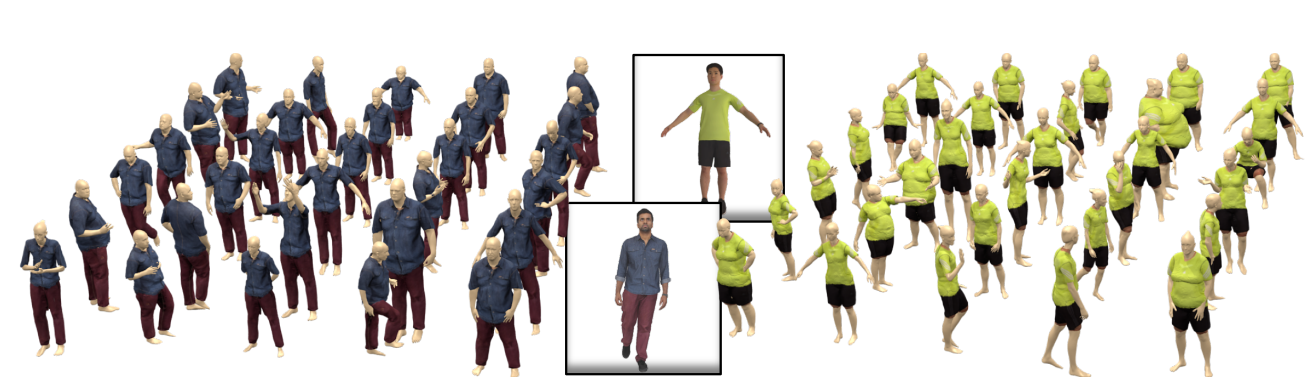
\includegraphics[scale=0.5]{Images/SizerPic/Sizer5.png}
  \caption{Viene utilizzato MGN per l'estrazione dei vestiti da un soggetto sorgente (immagine centrale) e successivamente questi abiti vengono messi su persone arbitrarie in diverse pose grazie a SMPL. I set corrispondono a quello maschile (sinistra) e quello femminile (destra)}
    \label{fig:Sizer5}
\end{figure}

\medskip\medskip\medskip\medskip\medskip\medskip\medskip\medskip\medskip


Gli studi sui vestiti sono tanti, per fare in modo che un essere umano possa indossare virtualmente un abito che si adatti realisticamente ai propri movimenti in base al tipo di tessuto che si vuole rappresentare, bisogna fare un lavoro di processing dal punto di vista della tassellazione non banale.
In queste esperienze si arriva ad avere una mesh poligonale irregolare, di conseguenza una volta ottenuta la segmentazione non è possibile utilizzare separatamente gli abiti rispetto al resto del modello.

\newpage

\subsection{Approcci 3D}

I lavori che partono da scansioni 3D o sequenze di scansioni 3D che sono stati presi in considerazione sono: BUFF, SizerNet e CAPE, ma di seguito vengono illustrati anche due ulteriori metodi rilevanti.

\subsubsection{SPSD}

In “A Layered Model of Human Body and Garment Deformation” (2015 - \url{https://ieeexplore.ieee.org/document/7035823}), viene presentato un framework per l’apprendimento di un modello a tre livelli: forma del corpo umano, posa e deformazione degli indumenti. Il modello di deformazione proposto (Shape and Pose Space Deformation, SPSD) fornisce un controllo intuitivo ed indipendente sui tre parametri, producendo deformazioni naturalistiche sia degli abiti sia del corpo umano. I layer di deformazione della forma e della posa del modello sono addestrati su un ampio dataset di 520 scansioni 3D di 115 soggetti umani (57 uomini e 57 donne) in varie pose (N. Hasler, C. Stoll, M. Sunkel, B. Rosenhahn and H. P. Seidel, "A Statistical Model of Human Pose and Body Shape", Computer Graphics Forum, vol. 28, no. 2, pp. 337-346, 2009.). Il layer della deformazione degli indumenti, invece, è addestrato su sequenze di mesh animate di attori vestiti e si basa su una tecnica per la stima della forma e della postura umana sotto i vestiti. Il contributo chiave di tale articolo è la considerazione delle deformazioni degli abiti come trasformazioni residue tra una mesh di un soggetto svestito ed una della stessa persona vestita.
L'inizializzazione della posa richiede un input manuale.


%\newpage

\subsubsection{BUFF}

In “Detailed, accurate, human shape estimation from clothed 3D scan sequences” (2017 - \url{https://arxiv.org/pdf/1703.04454.pdf}) si parte da scansioni statiche 3Dimensionali, o sequenze di scansioni 3D, e si cercano di stimare posa e forma al di sotto dei vestiti. Se tali scansioni contengono informazioni sul colore, queste vengono usate per dividere i vertici delle scansioni in pelle e indumento, altrimenti tutti i vertici vengono considerati appartenenti ai vestiti. Viene usato il metodo di segmentazione descritto in \url{https://www.researchgate.net/publication/318612942_ClothCap_Seamless_4D_Clothing_Capture_and_Retargeting}. Per rendere uniforme la funzione di costo, viene calcolata prima la distanza geodetica tra un punto e quello del tessuto più vicino, per poi applicare una funzione logistica per mappare i valori della distanza geodetica compresi tra 0 e 1 (Fig. 3 b). Il valore risultante viene propagato ai punti di scansione mediante nearest distance e utilizzato per pesare ogni residuo di scansione. In questo modo, i punti vicini al confine pelle-tessuto hanno un peso decrescente uniforme. Ciò rende effettivamente la funzione non discontinua (smooth) e robusta a segmentazioni imprecise.


\begin{figure}[ht!]
  \centering
  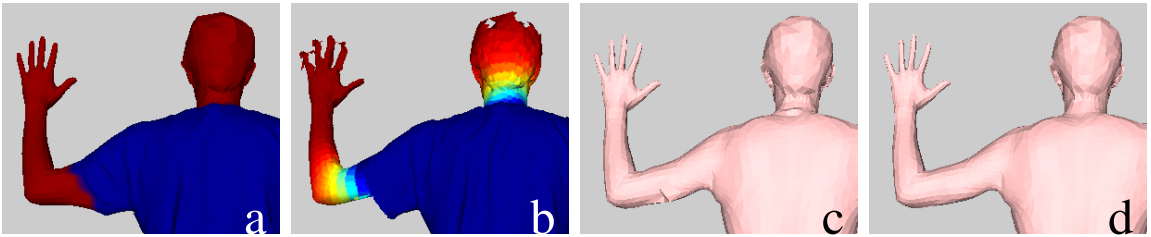
\includegraphics[scale=0.5]{Images/IntroductionPic/BUFF.png}
  \caption{Valore dei pesi dati alla pelle. \\ a) segmentazione ed allineamento (rosso: pelle, blu: vestiti) \\ b) distanza geodetica dal vertice del tessuto più vicino relativo all'allineamento \\ c) risultato 'sbagliato' con collo e braccio non generalizzato \\ d) risultato finale}
  \label{fig:BUFF}
\end{figure}

\medskip

Il dataset BUFF (\url{https://3dmd.com/tag/buff-dataset/}) contiene 11’054 clothed scans ad alta risoluzione con la corrispondente ground truth naked shape per ogni soggetto.

\newpage

\subsubsection{Sizer}

In “SIZER: A Dataset and Model for Parsing 3D Clothing and Learning Size Sensitive 3D Clothing” (\url{https://virtualhumans.mpi-inf.mpg.de/papers/tiwari20sizer/sizer.pdf}) ci si focalizza sulla vestibilità di vestiti virtuali su scansioni 3D del corpo. Gli indumenti interagiscono con il corpo in modo complesso, e la vestibilità è una funzione non lineare di taglia e shape del corpo, per cui simulare tale vestibilità non è banale. Viene introdotto il dataset SIZER (\url{http://virtualhumans.mpi-inf.mpg.de/sizer/}), un dataset di circa 2000 scansioni 3D di 100 persone che indossano 10 tipi di vestiario in taglie diverse (S, M, L, XL), registrazioni sul modello SMPL, scansioni segmentate in tipi di vestiario, categorie di vestiti e taglie.
Con SIZER viene addestrata una rete neurale, SizerNet, che permette di stimare e visualizzare la vestibilità dei vestiti in base alla taglia, la human body shape e l’indumento dati in input. L’addestramento di SizerNet necessita di un mapping tra le scansioni e mesh multi-strato - mesh separate per il corpo e per i capi di sopra e di sotto. Per fare ciò, c’è bisogno di segmentare le scansioni 3D, stimare la body shape senza vestiti e registrare gli indumenti attraverso il dataset ottenuto tramite una feature extraction effettuata mediante i metodi spiegati in “Bhatnagar, B.L., Tiwari, G., Theobalt, C., Pons-Moll, G.: Multi-garment net: Learning to dress 3d people from image” - 2019 http://virtualhumans.mpi-inf.mpg.de/mgn/ - e “ Pons-Moll, G., Pujades, S., Hu, S., Black, M.: ClothCap: Seamless 4D clothing capture and retargeting. ACM Transactions on Graphics 36(4)” - 2017 \url{https://virtualhumans.mpi-inf.mpg.de/papers/ponsmollSIGGRAPH17clothcap/ponsmollSIGGRAPH17clothcap.pdf}.
Dalle mesh multi-livello viene addestrato un codificatore in grado di mappare la mesh data in input ad un codice, ed un decodificatore che prende i parametri della forma del corpo di SMPL, la taglia dei vestiti dati in input e la taglia desiderata, per predire la vestibilità dei vestiti della taglia desiderata. Le scansioni, tuttavia, sono solo nuvole di punti, e analizzandoli (parsing) in una rappresentazione multi-layer al momento del test usando il metodo spiegato precedentemente (nel todo), richiede segmentazione, la quale può avere bisogno di un intervento manuale. Per questo è stata proposta anche ParserNet, la quale mappa automaticamente la registrazione di una singola mesh ad una mesh multi-layer con un solo passo feed-forward. ParserNet non solo segmenta la singola mesh registration, ma riparametrizza la superficie in modo da renderla coerente con i template dei vestiti più comuni.
La rappresentazione multi-layer di ParserNet permette dunque di modificare i vestiti direttamente da una mesh data in input, eliminando la necessità di una segmentazione delle scansioni.
Vengono quindi utilizzate: una rete neurale che predice i parametri relativi alla posa, una per predire i parametri della forma, ParserNet, che fa la segmentazione (riconosce il corpo e i singoli vestiti) e SizerNet, che modifica la taglia dei vestiti: prende in input una mesh 3D e restituisce in output corpi 3D svestiti ad alta qualità, mantenendo l’identità del soggetto.


\begin{figure}[ht!]
  \centering
  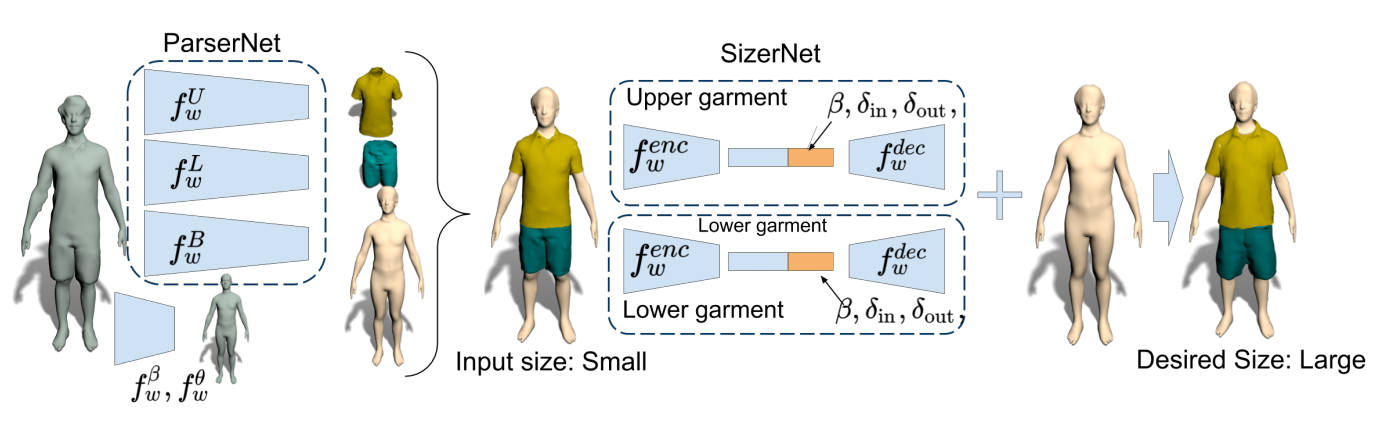
\includegraphics[scale=0.45]{Images/IntroductionPic/Sizer.png}
  \caption{Viene proposto un modello per stimare e visualizzare l'effetto che viene a formarsi vestendo capi condizionati dalla forma e dalla taglia del corpo. Per fare questo viene introdotto ParserNet $(f_{w}^{U}, f_{w}^{L}, f_{w}^{B})$, che prende una mesh precedentemente registrata da SMPL $M(\boldsymbol{\theta}, \boldsymbol{\beta}, \mathbf{D})$ come input e prevede i parametri SMPL $(\boldsymbol{\theta}, \boldsymbol{\beta})$ analizzando gli indumenti 3D ed utilizzando dei modelli predefiniti $T^{g}(\boldsymbol{\beta}, \boldsymbol{\theta}, \mathbf{0})$ prevedendo la forma del corpo che si cela sotto ai vestiti continuando a preservare i dati personali del soggetto. Viene inoltre proposto SizerNet, una rete encoder-decoder $\left(f_{w}^{\mathrm{enc}}, f_{w}^{\mathrm{dec}}\right)$ che ridimensiona il capo $\left(\delta_{\mathrm{in}}, \delta_{\mathrm{out}}\right)$ e lo adatta alla forma del corpo.  }
    \label{fig:Sizer}
\end{figure}

\newpage

\subsubsection{SMPL}
  
MPL, ovvero “Skinned Multi-Person Linear Model (\url{https://files.is.tue.mpg.de/black/papers/SMPL2015.pdf}), si pone come obiettivo quello di rappresentare corpi umani animati realistici che possano compiere diverse pose, deformandosi in maniera completamente naturale mantenendo però la fisionomia e la struttura del corpo umano che tutti noi conosciamo.

  \begin{figure}[ht!]
  \centering
  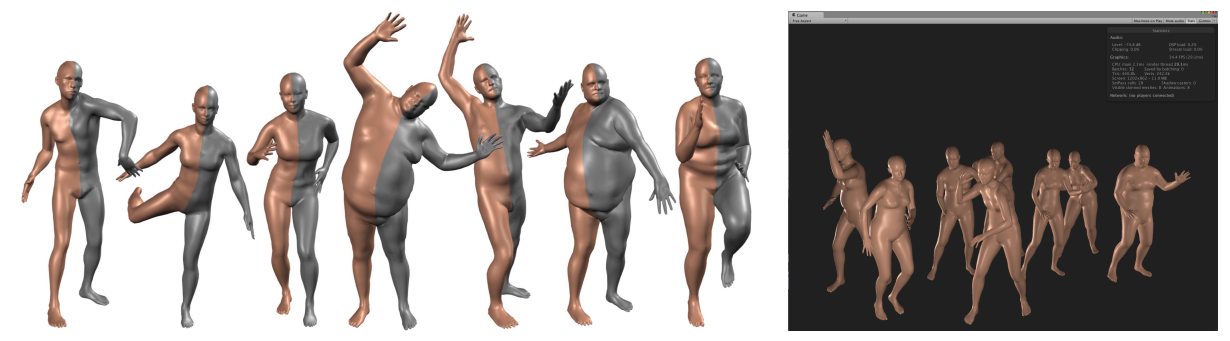
\includegraphics[scale=0.4]{Images/IntroductionPic/SMPL.png}
  \caption{SMPL è un modello realistico appreso della forma e della posa del corpo umano che è compatibile con i motori di rendering esistenti, consente
controllo dell'animatore ed è disponibile per scopi di ricerca. (a sinistra) Modello SMPL (arancione) adatto a mesh 3D della verità a terra (grigio). (a destra) Unità 5.0
screenshot del motore di gioco che mostra i corpi del dataset CAESAR animati in tempo reale.}
  \label{fig:SMPL}
\end{figure}

\medskip

Tali modelli devono essere precisi, facili da implementare, veloci da renderizzare e compatibili con i motori di editor/rendering preesistenti sul mercato. Per realizzare tutto sono necessarie molte blend shapes , molto problematiche da realizzare perché richiedono un enorme sforzo manuale e altrettanto investimento temporale. Per ovviare al problema, la comunità di ricerca scientifica si è concentrata sull’apprendimento di modelli statici come per esempio numerose scansioni dello stesso corpo in pose diverse. Inizialmente si è rivelata un’alternativa molto promettente ma, con l’avanzare delle tecnologie, questo metodo si è rivelato non compatibile con i vari software grafici presenti sul mercato e con i vari motori di rendering che utilizzano i metodi di skinning classici.
SMPL descrive, appunto, un modello del corpo umano che possa rappresentare una vasta gamma di pose, con variazioni dipendenti dalla posa stessa mostrando il funzionamento delle dinamiche dei tessuti molli mantenendo l’efficienza e la compatibilità con i motori di rendering esistenti.
I metodi tradizionali modellano il modo in cui i vertici sono correlati ad una struttura scheletrica sottostante. Il modello più utilizzato è senza ombra di dubbio il “Basic Linear Blend Skinning” (LBS) il quale è si supportato da tutti i game engines, nonché efficiente da renderizzare; sfortunatamente però produce deformazioni delle pose completamente irrealistiche rispetto alle articolazioni umane, producendo i famosi effetti “taffy” e “papillon”

\medskip

\begin{figure}[ht!]
  \centering
  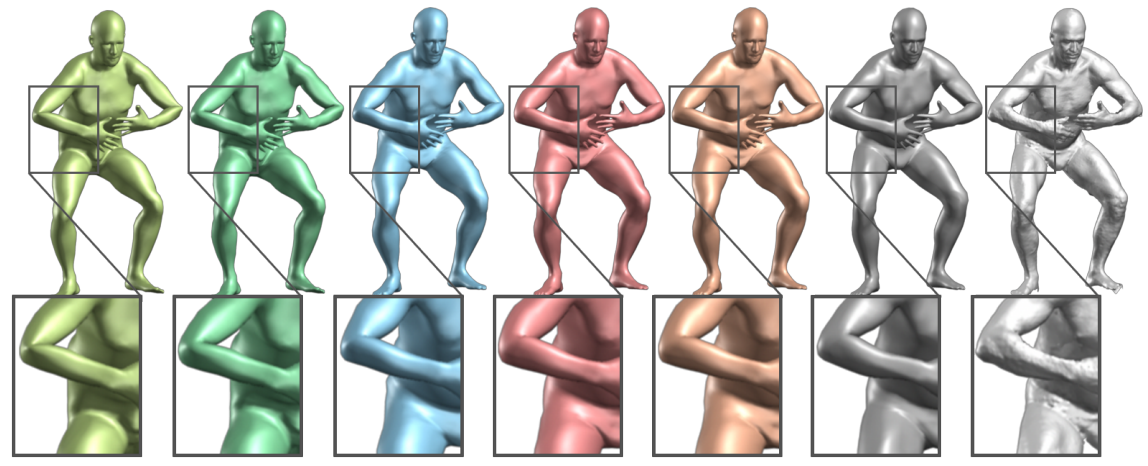
\includegraphics[scale=0.4]{Images/IntroductionPic/SMPL2.png}
  \caption{Modelli a confronto con verità di base. Questa figura definisce la codifica a colori utilizzata nel documento e nel video supplementare.
La mesh all'estrema destra (grigio chiaro) è una scansione 3D. Accanto ad essa (grigio scuro) c'è una mesh registrata con la stessa topologia del nostro modello. Chiediamo come
ben diversi modelli possono approssimare questa registrazione. Da sinistra a destra: (verde chiaro) Skinning blend lineare (LBS), (verde scuro) Skinning blend Dualquaternion (DQBS), (blu) BlendSCAPE, (rosso) SMPL-LBS, (arancione) SMPL-DQBS. Le regioni ingrandite evidenziano le differenze
tra i modelli al gomito destro e all'anca del soggetto. LBS e DQBS producono gravi artefatti su ginocchia, gomiti, spalle e fianchi.
BlendSCAPE ed entrambi i modelli SMPL si comportano allo stesso modo bene nell'adattare i dati.}
  \label{fig:SMPL2}
\end{figure}

\newpage

Un lavoro straordinario è stato dedicato sia ai metodi di skinning che cercano di migliorare questi effetti (Lewis et al. 2000; Wang and Phillips 2002; Kavan and Zˇ ara 2005; Merry et al. 2006; Kavan et al. 2008), sia per migliorare l’apprendimento di modelli corporei altamente realistici dai dati (Allen et al. 2006; Anguelov et al. 2005; Freifeld and Black 2012; Hasler et al. 2010; Chang and Zwicker 2009; Chen et al. 2013).
Nonostante gli enormi sforzi nell’implementazione di metodi, sono rimasti annidati molti problemi tra cui:
\begin{itemize}
\item mancanza di realismo
\item non funzionamento con i pacchetti esistenti
\item non rappresentazione di una discreta varietà di pose
\item non compatibilità con le pipeline grafiche standard
\item richiesto un notevole lavoro manuale
\end{itemize}

Contrariamente agli approcci precedenti, un obiettivo chiave del progetto SMPL è quello di rendere il modello del corpo il più semplice e standard possibile in modo che possa essere ampiamente utilizzato, mantenendo allo stesso tempo il  realismo di modelli basati sulla deformazione appresi dai dati. Nello specifico vengono implementate diverse blend shapes per correggere i limiti dello skinning tradizionale.
Blend shapes per identità, posa e dinamiche dei tessuti molli vengono combinate in modo additivo con un modello di riposo prima di essere trasformate da una blend skin.
Per imparare a riconoscere i vari portamenti del corpo, SMPL utilizza 1786 scansioni in alta risoluzioni con un'ampia varietà di pose.
Viene inoltre utilizzata la PCA (principal component analysis) per imparare i modelli lineari maschili e femminili dal dataset CAESAR (con approssimativamente 2000 scansioni maschili e femminili). 

\medskip

Inizialmente viene registrata una mesh template per ogni scansione e ne viene quindi normalizzata la posa (processo molto importante quando si sta imparando da un modello vertex-based shape).


\medskip

Successivamente viene allenato il modello SMPL in diversi modi e confrontato quantitativamente con un simile modello BlendSCAPE [Hirshberg et al. 2012], allenato anch’esso con gli stessi dati.
I 2 modelli vengono poi valutati qualitativamente con animazioni e quantitativamente utilizzando delle mesh mai viste durante la fase di training.
SMPL e BlendSCAPE vengono adattati a queste nuove mesh e viene fatta un’analisi sugli errori di vertice.
Sono state esplorate principalmente 2 varianti del modello SMPL:
\begin{enumerate}
\item la prima utilizzando LBS (linear blend skinning)
\item la seconda usando DQBS (Dual-Quaternion blend skinning)
\end{enumerate}

\medskip

Risulta che un modello skinned vertex-based come SMPL è molto più accurato rispetto a un modello deformation-based come il BlendSCAPE (avendo svolto la fase di training sugli stessi dati).
Il modello SMPL è stato anche esteso per catturare e modellare la dinamica dei tessuti “molli” adattando il Dyna model [Pons-Moll et al. 2015].
Il risultante modello “Dynamic-SMPL” o DMPL, viene addestrato dallo stesso set di dati di mesh 4D di Dyna. DMPL, a differenza di Dyna, si basa su vertici anziché su deformazioni triangolari. Successivamente vengono calcolati ed analizzati gli errori di vertice tra le mash SMPL e Dyna, e tramite l’utilizzo di PCA viene ridotta la dimensionalità producendo delle blend shapes dinamiche. Un modello di tessuto “molle” viene addestrato sulla base di velocità angolari e deformazioni dinamiche con fatto in [Pons-Moll et al. 2015]. In questo genere di tessuti, la dinamica dipende fortemente dalla forma del corpo; DMPL viene addestrata usando corpi con variabili indici di massa corporea e concentrandosi nel training che dipenda fortemente dai movimenti e pose del corpo stesso.

\newpage

\paragraph{Linear Blend Skinning}~

\medskip

La skin blend lineare è l'idea di trasformare i vertici all'interno di una singola mesh mediante una (blend) di più trasformazioni. Ogni trasformazione è la concatenazione di una "matrice di legame" che porta il vertice nello spazio locale di un dato "osso" e una matrice di trasformazione che si sposta dallo spazio locale di quell'osso in una nuova posizione.
Verrà usata una shader di questo tipo:

\medskip

\begin{figure}[ht!]
  \centering
  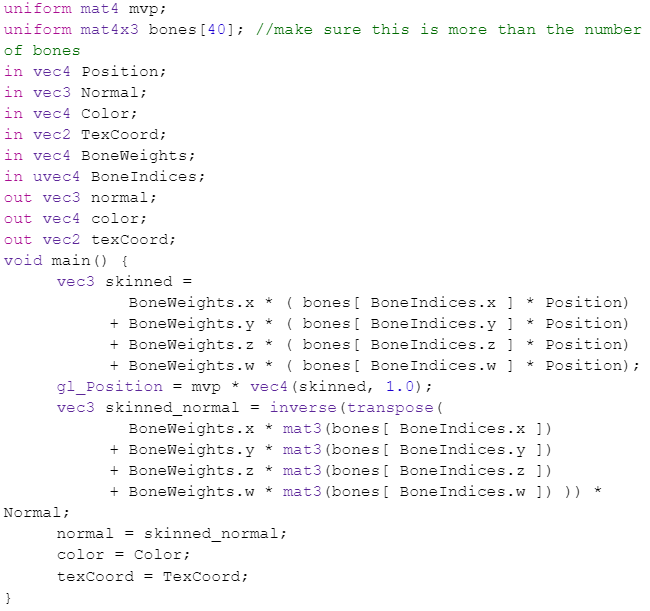
\includegraphics[scale=0.9]{Images/IntroductionPic/LBShape.png}
  \label{fig:LBShape}
\end{figure}

\newpage

\paragraph{Blend Shapes}~

Le Blend Shapes permettono di trasformare la forma di un oggetto in un altro, più nello specifico consentono di trasformarne la superficie stessa.
Per esempio, un uso ricorrente delle Blend Shapes riguarda l’animazione facciale:


\begin{figure}[ht!]
  \centering
  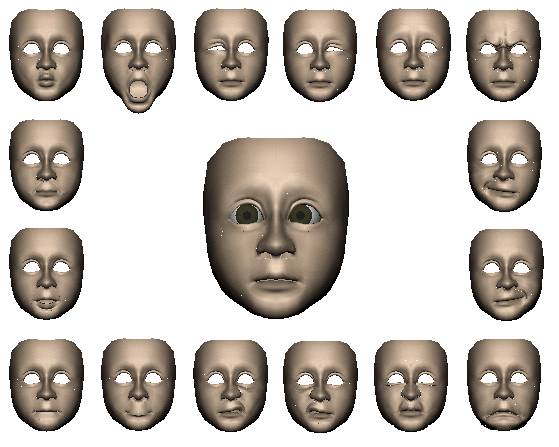
\includegraphics[scale=0.6]{Images/IntroductionPic/BlendShapes.png}
  \caption{Quando viene creata una blend shape, si identificano uno o più oggetti che si vogliono deformare. Gli oggetti utilizzati per “prendere” la forma interessata sono chiamati oggetti target, mentre l'oggetto deformato è chiamato oggetto base.}
  \label{fig:LBShape}
\end{figure}

\subsubsection{CAPE}

CAPE (\url{https://cape.is.tuebingen.mpg.de/media/upload/CAPE_paper.pdf}) è un modello generativo strutturato su grafi a base di reti neurali convoluzionali per la realizzazione di mesh tridimensionali specifiche per l’adattamento dei vestiti al corpo umano. È compatibile con i più famosi modelli che analizzano il corpo umano, come per esempio SMPL,  e può essere generalizzato a particolari pose e movimenti del corpo. È progettato per essere "plug-and-play" per molte applicazioni che già utilizzano SMPL.
Il dataset di CAPE fornisce delle mesh registration nel metodo SMPL quadridimensionali di scansioni relative a persone vestite, insieme a scansioni veritiere delle forme del corpo spoglie di ogni vestito.


\medskip

Per modellare i corpi vestiti, CAPE li fattorizza in due parti: 
\begin{enumerate}
\item corpo con pochi vestiti
\item layer vestito rappresentato come un offset dal corpo
\end{enumerate}

\medskip

Classificando in questo modo, CAPE è in grado di estendere in maniera completamente naturale SMPL ad una classe di tipi di abbigliamento trattando il vestito come una shape aggiuntiva.
Grazie alla rapida diffusione di SMPL, l’obiettivo di CAPE è diventato quello di estendere i metodi implementati da SMPL in maniera coerente agli attuali usi.

\newpage

Come già precedentemente spiegato, SMPL è un modello che fattorizza la superficie del corpo nei parametri forma $(\beta)$ e posa $(\theta)$.
Come mostrato nella figura sottostante (sezione a,b), l'architettura di SMPL inizia con il template di una mesh triangolare $\bar{T}$, definita da $N=6890$ vertici. Dopo aver dato al modello i parametri forma e posa $(\beta, \theta)$, vengono aggiunti al template gli offset 3D corrispondenti a deformazioni dipendenti 

\medskip 

\begin{itemize}
\item dalla forma $\left(B_{S}(\beta)\right)$
\item dalla posa $\left(B_{P}(\theta)\right)$
\end{itemize}

La posa della mesh risultante viene ottenuta usando una funzione di skinning W. Formalmente abbiamo:

\medskip

\begin{equation}
\begin{aligned}
T(\beta, \theta) &=\bar{T}+B_{S}(\beta)+B_{P}(\theta) \\
M(\beta, \theta) &=W(T(\beta, \theta), J(\beta), \theta, \mathcal{W})
\end{aligned}
\end{equation}

\medskip

dove la funzione di sfumatura della pelle $W(-)$ ruota i vertici $T$ della posa a “riposo” intorno ai giunti tridimensionali $J$ (calcolati grazie a $\beta$), li “leviga” linearmente grazie ai pesi di fusione  $W$ e restituisce i vertici della nuova posa $M$. 

\medskip

\begin{figure}[ht!]
  \centering
  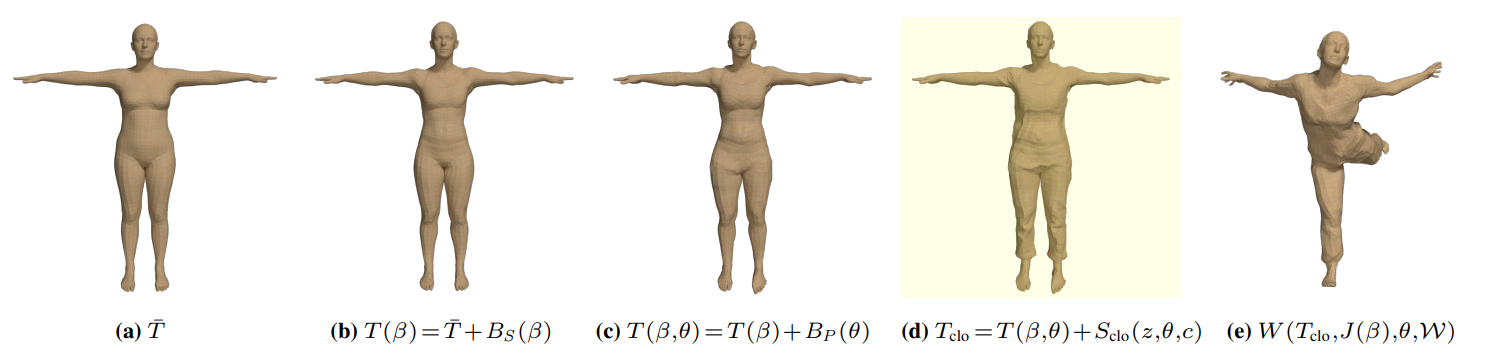
\includegraphics[scale=0.4]{Images/IntroductionPic/CAPE.png}
  \caption{Il contributo principale viene evidenziato dallo sfondo giallo.\\
  Partendo da SMPL, CAPE (a) aggiunge linearmente gli offset forniti da (b), la forma del corpo individuale $(/beta)$ e (c) la posa $(/theta)$; da notale da deformazione sui fianchi e sui piedi per via della posa. (d) Viene inoltre aggiunto uno strato di abbigliamento c e una variabile di forma z. (e) i vertici vengono computati usando l'equazione di skinning di SMPL.}
  \label{fig:CAPE}
\end{figure}

\medskip

SMPL aggiunge dei livelli (strati) di deformazione lineare ad uno strato iniziale composto dalla posa “standard” del corpo.
Successivamente, CAPE definisce l’abbigliamento come  un livello extra di offset dal corpo e lo aggiunge sopra alla mesh realizzata da SMPL, come in Fig. 2 (d).

\newpage

\paragraph{Architettura della rete}~
\medskip

Come mostrato nell'immagine sottostante, il modello è costituito da un generatore
G con architettura encoder-decoder e discriminatore D. Vengono inoltre utilizzate reti ausiliarie C1, C2 per gestire il problema del condizionamento. La rete è differenziabile ed è trainata end to end.

\begin{figure}[ht!]
  \centering
  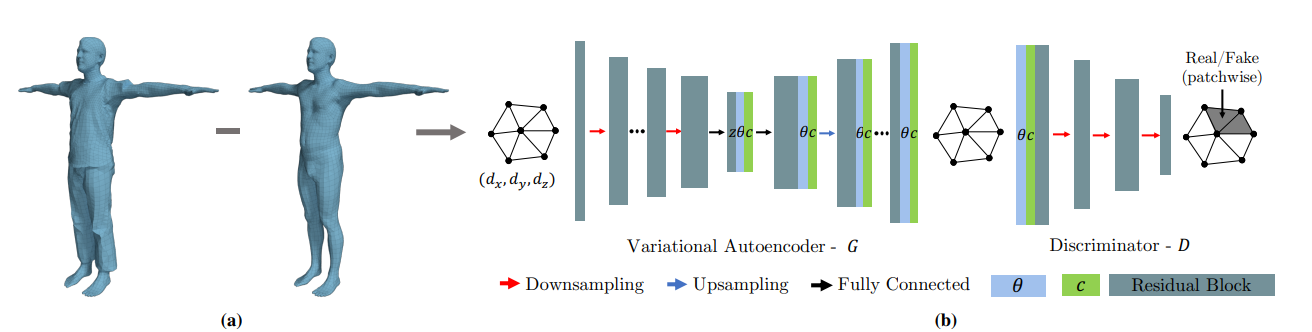
\includegraphics[scale=0.4]{Images/IntroductionPic/CAPENetwork.png}
  \caption{(a) calcola gli spostamenti dai dati di scanzione sottraendo la minima forma del corpo dalla mesh del corpo vestito (b) }
  \label{fig:CAPENetwork}
\end{figure}


Per semplicità, in questa sezione verrà utilizzata la seguente notazione.

\medskip

$x$: i vertici $\nu_d$ del grafo di spostamento in ingresso; \\
$X$: vertici del grafo ricostruito;\\
$\theta$ e $c$: la posa ed il
vettore di condizionamento in base al capo\\
$z$: il codice latente.

\medskip

\textbf{Generatore di grafici}. Viene costruito il generatore di grafi seguendo una rete di tipo VAE-GAN. Durante l'allenamento, un encoder Enc(·)
prende lo spostamento x, estrae le sue caratteristiche attraverso più strati convoluzionali del grafico e lo mappa sul codice latente a bassa dimensione z. Un decoder viene addestrato per ricostruire il grafico di input $\hat{x}=D \operatorname{ec}(z)$ da z. Sia l'encoder che il decoder sono reti neurali feed-forward costruite
con strati convoluzionali mesh. I livelli lineari sono usati alla fine dell'encoder e all'inizio del decoder.

\medskip

L'impilare i livelli convoluzionali provenienti dal grafico genera una perdita di features negli strati più profondi. Questo è un gravissimo problema, soprattutto nell'ambito del clothing generation perchè alcuni dettagli, come per esempio le pieghe, tendono a scomparire.Pertanto, vengono migliorati gli strati di convoluzione del grafico standard con connessioni residue, che consentono l'uso di caratteristiche di basso livello da quello di input, se necessario.

\medskip

Al momento del test, l'encoder non è necessario. Invece, z viene campionato dalla distribuzione a priori gaussiana e dal decodificatore
funge da generatore di grafici: $G(z) = Dec(z)$.

\medskip

\textbf{Discriminatore Patchwise}. Per migliorare ulteriormente i dettagli nella fase di ricostruzione, viene introdotto un discriminatore patchwise D per i grafici, che ha mostrato successo nel dominio dell'immagine.

Invece di guardare l'intero grafico generato, il discriminatore classifica solo se la patch è vera o falsa in base alla sua struttura locale. Intuitivamente questo incoraggia il discriminatore a concentrarsi solo sui
dettagli più raffinati e per quanto riguarda la forma 'globale', se ne occupa la reconstruction loss.

\medskip

Viene implementato il grafico patchwise-discriminator utilizzando quattro grafici di convoluzione-sottocampionamento a
blocchi. Successivamente viene aggiunto una perdita reale/fasulla discriminante per ciascuno dei vertici di output.  Questo abilita il discriminatore
a catturare una patch di nodi vicini nel grafico ricostruito e classificarli come reali / falsi.

\medskip

\textbf{Modello condizionale}. Si condiziona la rete con bodypose $\theta$ e abbigliamento di tipo c. I parametri di posa SMPL sono
nella rappresentazione asse-angolo e sono difficili da apprendere per la rete neurale.
Pertanto vengono trasformati i parametri di posa in matrici rotazionali usando l'equazione di Rodrigues.
Entrambe le condizioni v engono prima passate attraverso una piccola rete di incorporamento completamente connessa, $C_{1}(\theta), C_{2}(c)$, rispettivamente, in modo da bilanciare la dimensionalità di apprendimento delle features del grafico e di condizionamento.

\medskip

Si sperimenta, inoltre, diversi modi di condizionare il generatore di mesh: 

Concatenazione nello spazio latente; aggiungere le features delle condizioni alle features del grafico in tutti i nodi del generatore; e la combinazione dei due. Risulta che la strategia combinata funziona meglio in termini di capacità di rete e di effetto del condizionamento.


\paragraph{Ricostruzione di persone 3D}~

La ricostruzione di esseri umani 3D da immagini e video 2D è un classico problema di visione artificiale.
La maggior parte degli approcci generano mesh del corpo 3D dalle immagini, ma non dai vestiti.
Questo tipo di approccio ignora completamente dettagli delle immagini che potrebbero essere utili ai fini dell’obiettivo stesso.
Per ricostruire i corpi con i vestiti addosso, i più famosi metodi utilizzano rappresentazioni di profondità volumetriche  o biplanari per modellare il corpo e gli abiti nel loro insieme.
Un altro gruppo di metodi si basa sul SMPL.
Rappresentano l'abbigliamento come uno strato sfalsato rispetto al corpo sottostante come proposto in ClothCap (gruppo 2 nella Tabella 1).

\paragraph{Modelli parametrici per corpi e abiti 3D}~

I modelli statistici tridimensionali del corpo umano ricavati dalle scansioni 3D catturano la forma e la posa, rendendoli un elemento fondamentale per molteplici applicazioni.
Nella maggior parte dei casi, tuttavia, le persone sono vestite quando questi modelli non rappresentano l’abbigliamento stesso.
Inoltre, mentre ci muoviamo, i vestiti cambiano forma producendo pieghe che a loro volta possono mutare in molti modi diversi.
Sebbene esistano modelli di abbigliamento appresi da dati reali, pochi di questi si adattano a pose non comuni. Ad esempio, Neophytou e Hilton apprendono un modello basato sulla stratificazione degli indumenti sulla base di SCAPE da sequenze dinamiche, anche se la generalizzazione a nuove pose non è ancora stata dimostrata.
Un approccio concettualmente diverso deduce i parametri di un modello di abbigliamento da sequenze di scansioni tridimensionali.
In questo caso è possibile generalizzare a nuove pose creando, però, il grave problema dell’interferenza e, a differenza di CAPE, il simulatore fisico risultante non è differenziabile rispetto ai parametri stessi.

\medskip

Il dataset CAPE è facilmente scaricabile, sono approssimativamente 49GB.
Per ottenere i dataset di Buff (\url{https://arxiv.org/pdf/1703.04454.pdf}) e SIZER bisogna necessariamente contattare gli owners.
Per Buff bisogna inviare una email seguendo le istruzioni del seguente link \url{http://buff.is.tue.mpg.de/downloads}. Per quanto riguarda SIZER, invece, qui c'è un form da compilare \url{https://docs.google.com/forms/d/e/1FAIpQLSddBep3Eif1gI-6IhaZybBDoR-_H_QW1NST0JV5vviauvPNTA/viewform}, oppure si può inviare una mail a \url{gtiwari@mpi-inf.mpg.de} per ottenere sia il dataset che il modello, come indicato qui \url{https://github.com/garvita-tiwari/sizer}.

\medskip

La cattura, ricostruzione e la modellazione di abiti sono 3 punti che sono stati ampiamente studiati negli ultimi decenni.
La tabella 1 mostra i più famosi metodi degli ultimi anni categorizzati in due classi principali: (1) metodi di ricostruzione e cattura e (2) modelli parametrici, dettagliati come segue.

\medskip

\begin{figure}[ht!]
  \centering
  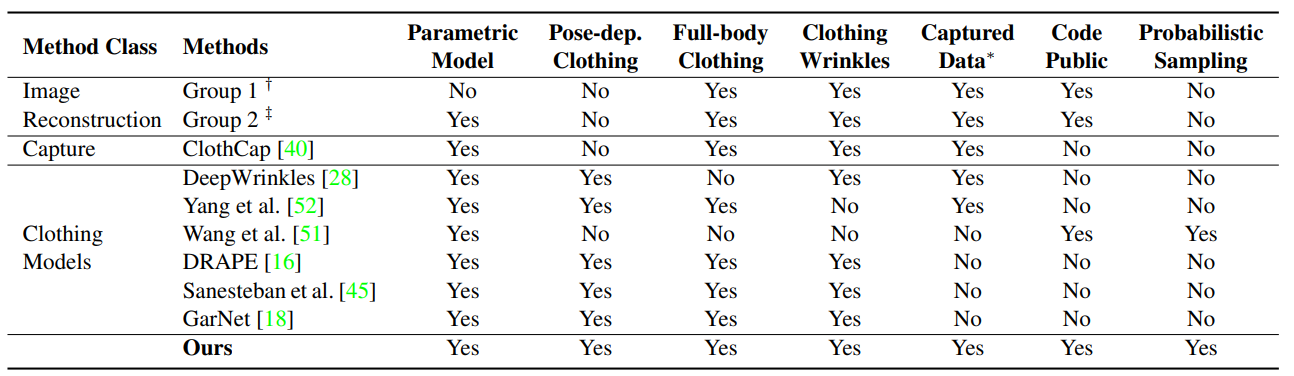
\includegraphics[scale=0.4]{Images/IntroductionPic/CAPETabel.png}
  \caption{Selezione di metodi correlati. Esistono due principali classi di metodi di abbigliamento 3D: (1) metodi di ricostruzione e acquisizione basati su immagini e (2) abbigliamento
modelli che prevedono la deformazione in funzione della posa. All'interno di ciascuna classe, i metodi differiscono in base ai criteri nelle colonne.}
  \label{fig:CAPETabel}
\end{figure}

\medskip

\subsubsection{ClothCap}

In “ClothCap: Seamless 4D Clothing Capture and Retargeting” 

(\url{https://virtualhumans.mpi-inf.mpg.de/papers/ponsmollSIGGRAPH17clothcap/ponsmollSIGGRAPH17clothcap.pdf})

\medskip

L’idea di questo metodo, invece, riguarda un approccio data-driven alla cattura dei vestiti (ClothCap); processando abbigliamento dinamico vestito su persone da scansioni quadridimensionali in modo da poter essere computato in maniera più semplice dei tradizionali metodi e applicato su avatar virtuali.

\medskip

Viene catturata la geometria dell’abito su un corpo in movimento, viene stimata sia la forma del corpo che la sua morfologia sotto i vestiti per poi segmentare ed estrarre i vari capi.
I nuovi capi catturati in questo modo vengono assegnati successivamente a nuove persone, anche con pose differenti.

\medskip

Per fare ciò, viene sviluppato un modello multi-parte orientato alle mesh dimostrando come segmentare, rintracciare e recuperare la forma di un capo a partire da sequenze di scansioni tridimensionali.

\medskip

\begin{figure}[ht!]
  \centering
  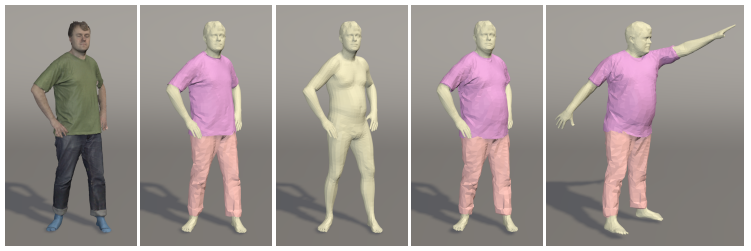
\includegraphics[scale=0.5]{Images/SizerPic/Sizer6.png}
  \caption{Da sinistra a destra: (1) Un esempio di scansione con texture 3D che fa parte di una sequenza 4D. (2) Il modello di mesh allineato in più parti, sovrapposto al
corpo. (3) La forma minimamente vestita (MCS) stimata sotto i vestiti. (4) Il corpo irrobustito e vestito con gli stessi abiti. Si noti che l'abbigliamento
si adatta in modo naturale alla nuova forma del corpo. (5) Questa nuova forma del corpo si pone in una posa nuova, mai vista. Questo illustra come ClothCap supporta una gamma di
applicazioni relative all'acquisizione, alla modellazione, al retargeting, alla posa e alla prova di abbigliamento}
    \label{fig:Sizer6}
\end{figure}

\medskip

I metodi di cattura esistenti soffrono di bassa risoluzioni, forme statiche, troppa semplicità nei movimenti del corpo, cattura di solo un capo di abbigliamento o la non completa segmentazione dei vestiti.
Conseguentemente, i problemi chiave da risolvere includono l’acquisizione di alta qualità, la segmentazione, il tracciamento della forma e della superficie così come la stima della morfologia del corpo e come questo stia posando.

\medskip

Come input, viene data una nuvola di punti (con texture).

\medskip

La rappresentazione multi-mesh è consistente con il modo in cui l’abito viene indossato, modellando e adattando il continuo cambiamento di visibilità delle superfici del vestito nel tempo.
Inoltre permette di affrontare i problemi di segmentazione e tracciamento in un quadro coerente. In questo modo vengono segmentati automaticamente gli abiti dalle scansioni quadridimensionali usando informazioni sia riguardanti l’aspetto che la forma (Fig. 1 (2)) utilizzando un campo casuale di Markov 

\url{https://www.dsu.univr.it/documenti/Tesi/allegato/allegato517081.PDF}

\medskip

Dati gli abiti segmentati, viene adattato un set di modelli multiparte basati a mesh alle scansioni, mettendoli in corrispondenza nel tempo e stimando così la forma sottostante del vestito in forma minimale

\medskip

La filosofia di questo metodo sposta l’attenzione dalla simulazione alla cattura dei vestiti.
Le mesh dei vestiti estratte automaticamente sono naturalmente associate ad un modello corporeo articolato sottostante (SMPL (Loper et al. 2015)).
Grazie a questa tecnologia si è in grado di cambiare la morfologia del corpo come mostrato in (Fig. 1 (4)), oppure trasferire direttamente gli indumenti ad un nuovo corpo in maniera completamente automatica.
è vero che l’acquisizione del modello riguardante le pieghe non è completamente realistico; tuttavia l’aspetto visivo ottenuto è più che sufficiente per molte applicazioni try-on.


\medskip

In sintesi, ClothCap getta le basi per la modellazione degli abiti, affrontando problemi complessi relativi alla segmentazione e tracciamento di scansioni quadridimensionali.
In maniera più dettagliata, contribuisce a 
\begin{itemize}
\item metodo automatico per segmentare le sequenze di scansioni tridimensionali sfruttando un modello corporeo
\item un metodo di tracciamento del modello multi-mesh
\item una tecnica per riorientare il tessuto in maniera dinamica ad una nuova morfologia corporea
\end{itemize}


\medskip

L’intero metodo viene dimostrato estraendo diverse tipologie di abiti tra cui pantaloni lunghi, t-shirt e pantaloncini su un’ampia varietà di persone mentre eseguono movimenti non banali (complessi). Viene inoltre dimostrato che il metodo funziona per le gonne pur avendo una diversa topologia rispetto al corpo.

\medskip

\begin{figure}[ht!]
  \centering
  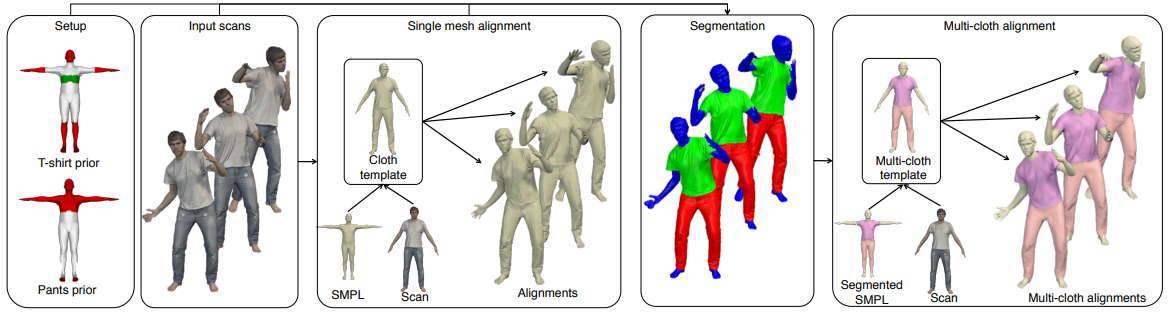
\includegraphics[scale=0.5]{Images/SizerPic/Sizer7.png}
  \caption{Sono necessari tre passaggi principali per ottenere allineamenti multitessuto: allineamento mesh singola, segmentazione della scansione e allineamento multitessuto. Multi-tessuto
gli indumenti di allineamento possono essere facilmente retargettati a nuove forme.}
    \label{fig:Sizer7}
\end{figure}

\medskip

ClothCap si basa su quattro steps principali:

\medskip

\begin{itemize}
    \item \textbf{\textit{Step 0: Installazione}}. Per catturare una specifica classe di abiti è necessario definire il numero di capi “Ngarm”  e istanziare una priorità spaziale relativamente bassa per intuire in quale parte del corpo gli abiti potrebbero trovarsi. Questo processo è molto grezzo e conseguentemente facile da realizzare. Inizialmente vengono trattati vestiti la cui topologia è facilmente mappabile al corpo per poi venire esteso ad un più ampio campo di vestiti con topologie via via più complicate come per esempio le gonne.
    Come modello del corpo viene utilizzato l’SMPL. (Loperet al. 2015).
    Nello specifico, per un soggetto, viene stimata una MCS (minimally clothed shape) ovvero la morfologia approssimativa del soggetto senza vestiti.
    L’MCS potrebbe essere stimato utilizzando una tecnologia esistente (Zhang et al. 2017) ma, dal momento che ClothCap acquisisce scansioni quadridimensionali dal soggetto, l’acquisizione di un’ulteriore scansione per inquadrare gli abiti “di base” richiederebbe minimo sforzo a livello computazionale e tempistico. Quindi viene allineato il modello del corpo insieme alla scansione dei vestiti basilari per ottenere l’ MCS. Infine ClothCap assume che tutte le sequenze di scansione partano (più o meno) con una posa alla “A”.
    \item \textbf{\textit{Step 1: Segmentazione}}.
    Le scansioni quadridimensionali includono geometria e informazione riguardante il colore e, ovviamente, contengono anche rumore e mancanza di dati. Risulta, quindi, difficile segmentare queste scansioni grezze pertanto il problema viene analizzato in due sottoproblemi:
    \begin{itemize}
        \item \textbf{\textit{Step 1a: Allineamento a mesh singola}}. Come primo passo viene allineato alle sequenze scansionate il modello del corpo umano fornito da SMPL. Successivamente ClothCap deforma il modello in modo da adattarlo al meglio ai dati osservati e inizializzare ciascun frame con il risultato del frame precedente. L’output di questo step è una sequenza registrata a bassa risoluzione di meshes.
        \item \textbf{\textit{Step 1b: Segmentazione}}. Attraverso l’utilizzo combinato della priority segmentation e un campo casuale Markoviano è possibile segmentare ogni frame della sequenza. Ciò fornisce una segmentazione sia dei singoli allineamenti della mesh sia una segmentazione basata sui vertici delle scansioni. Quindi grazie all’allineamento segmentato della singola mesh del primo frame (che, come citato sopra, si trova approssimativamente in una posa ad “A”) è possibile definire un template che determini la topologia del capo (ma non la geometria). Infine vengono scartati gli allineamenti della singola mesh.
        
        
    \end{itemize}
    \item \textbf{\textit{Step 2: Allineamento multitessuto}}.
    Il template segmentato dell’abito viene deformato in	modo da adattarsi alla scansione segmentata del primo fotogramma in modo da ottenere un modello multitessuto che è in grado di acquisire sia la topologia che la geometria dei capi e del corpo umano. Con questo tipo di allineamento ogni vestito viene tracciato per combaciare con i dati della scansione segmentata. Questa ottimizzazione implementa un parametro per regolarizzare i bordi del capo come per esempio nelle braccia, sul collo, nella vita e nelle caviglie. Inoltre un ulteriore parametro viene dedicato allo smoothing degli abiti. Questo step genera multi tessuti allineati alle scansioni, ovvero deformazioni del template multitessuto originale. Ne conclude che ogni abito in ogni fotogramma è allineato ad un template comune.
    \item \textbf{\textit{Step 3: Reindirizzamento}}. Per prima cosa bisogna considerare la sorgente di una persona che si sta muovendo con abiti che vogliamo reindirizzare.
    Da questa sequenza viene stimato l’MCS e computato un allineamento multitessuto; questo, però, non è sufficiente per l’operazione di reindirizzamento.
    Nella fase di preparazione viene stimata la morfologia di una persona svestita in un determinato lasso di tempo che potrebbe discostarsi dal MCS e viene stimato come il vestiario si possa adattare a questa nuova forma del corpo nella posa a “T”. Questa operazione viene svolta per ogni singolo fotogramma nella sequenza sorgente.
    Il reindirizzamento di un capo prevede 2 steps:
    \begin{itemize}
        \item preparazione
        \item vestizione 
    \end{itemize}
    
\end{itemize}



\medskip

\begin{figure}[ht!]
  \centering
  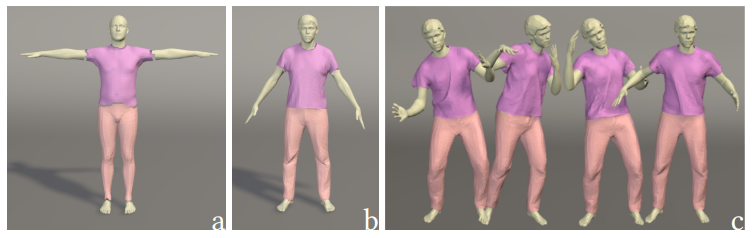
\includegraphics[scale=0.5]{Images/SizerPic/sizer8.png}
  \caption{modello di tessuto segmentato automaticamente: definisce il
solo topologia dell'indumento; cioè, quali vertici appartengono a ciascuna parte di stoffa. (b)
il modello multi-tessuto acquisisce sia la geometria che la topologia. Questo è calcolato
per ogni nuovo soggetto e capo e cattura la geometria di ciascuno
indumento. (c) gli allineamenti multi-tessuto sono deformazioni del multi-telo
modello per adattarsi a ogni fotogramma della sequenza.}
    \label{fig:Sizer8}
\end{figure}

\medskip

\newpage





























 









%\chapter{Obiettivi}
\section{Obiettivi}

Dalla conoscenza ottenuta durante la fase di ricerca della letteratura, sono emersi i seguenti obiettivi:

\begin{itemize}
\item ottenere le mesh dei singoli vestiti partendo da scansioni 3D
\item animare delle scansioni
\item animare i vestiti in real time
\end{itemize}

\medskip
Tali obiettivi possono essere accorpati nei seguenti macroargomenti:

\medskip

\begin{itemize}
\item Ricostruzione 3D. \\ Oltre a migliorare la pipeline 3D, è fondamentale il processo di delighting, cioè ricavare il colore di un oggetto indipendentemente dalle condizioni di luce ambientale.
\item Modelli deformabili. \\ Si intende lavorare sui corpi umani e vedere come i modelli si deformano, compresa la componente del vestito. L’obiettivo è dunque di separare la componente del corpo e quella del vestito vedendo l’indumento come un offset dai vertici del corpo umano. Partendo da una immagine comprendente un soggetto vestito, l’idea è quella di avere il modello 3D del corpo umano nudo e quello delle componenti del vestito. Un problema che si può riscontrare, però, è la limitatezza della tipologia di vestiti presi in considerazione solitamente.


\end{itemize}

\medskip

Questo capitolo sulla modellazione dei vestiti è ciò che ci interessa maggiormente: si può ricavare la modellazione del vestito a partire dal reale, cioè dall’osservazione di qualcuno che indossa tali indumenti, o, in alternativa, si può lavorare direttamente sulle immagini o su scansioni 3D di soggetti vestiti, in modo da non dover avere l’onere di gestire la parte di proiezione sull’immagine, andando a lavorare sulla parte di sola modellazione.
Una volta ottenute le mesh separate, bisogna re-mesharle per applicare algoritmi di deformazione di vestiti.

\medskip

I modelli tridimensionali del corpo umano sono ampiamente utilizzati
nell'analisi della posa e del movimento umano. I modelli esistenti, tuttavia, vengono processati da scansioni 3D con abiti di base, non riuscendo quindi a generalizzare la complessità delle persone che indossano qualcosa di più dettagliato, non riuscendo a studiare il modello nella sua interezza.
Inoltre, gli attuali modelli mancano della forza espressiva necessaria per rappresentare la complessa geometria non lineare di indumenti dipendenti dalla posa delle forme. 
Modellare ed analizzare come l’abbigliamento 3D si adatta e interagisca con il corpo umano in funzione di diverse strutture porta ad avere numerose applicazioni nel settore tecnologico odierno, in quanto parte di una consistente fetta applicativa relativa ai contenuti 3D (come per esempio film, videogiochi, settore AR/VR etc..).
Al giorno d’oggi è molto “rischioso” acquistare un capo online, in quanto non è possibile provarlo e vedere come viene calzato.
Proprio per questo motivo la vendita di vestiti sul web è uno tra i pochi settori che non è ancora riuscito a contrastare la controparte fisica: le persone hanno bisogno di provare capi di persona.
Si stima che i rivenditori di abiti online subiscano perdite per oltre 600 miliardi di dollari ogni anno a causa  di vendite tornate indietro: è difficile acquistare abiti online senza poterli provare.
%\chapter{SIZER: dataset e modello per l’analisi e l'apprendimento dell’abbigliamento 3D size sensitive}
\section{SIZER: dataset e modello per l’analisi e l'apprendimento dell’abbigliamento 3D size sensitive}

Esistono numerosi modelli nell’ambito dell’abbigliamento 3Dimensionale, progettati ed ottimizzati grazie a database costruiti su basi di dati reali.  
Nessuno di questi, però, è in grado di implementare la funzione di “deformare” l’abito in base alla taglia.

\medskip

\begin{itemize}
\item SizerNet in grado di prevedere le deformazioni 3D elaborate in tempo reale degli abiti condizionate in base ai parametri del corpo umano ed alle dimensioni dell’indumento 
\item ParserNet con l’obiettivo di decifrare e dedurre la struttura dei vestiti (e la loro forma), distinguendoli dal corpo umano tramite un singolo passaggio data una mesh in input.

\end{itemize}

\medskip

SizerNet apre la possibilità di stimare e visualizzare nel dettaglio la vestibilità di un indumento nelle sue varie taglie mentre ParserNet permette di modificare vestiti relativi alla mesh di input in maniera diretta e precisa, eliminando la necessità di scannerizzare le singole segmentazioni, problema molto impegnativo già in sé.

\medskip

In “SIZER: A Dataset and Model for Parsing 3D Clothing and Learning Size Sensitive 3D Clothing” (\url{https://virtualhumans.mpi-inf.mpg.de/papers/tiwari20sizer/sizer.pdf}) ci si focalizza sulla vestibilità di vestiti virtuali su scansioni 3D del corpo. Gli indumenti interagiscono con il corpo in modo complesso, e la vestibilità è una funzione non lineare di taglia e shape del corpo, per cui simulare tale vestibilità non è banale. Viene introdotto il dataset SIZER (\url{http://virtualhumans.mpi-inf.mpg.de/sizer/}), un dataset di circa 2000 scansioni 3D di 100 persone che indossano 10 tipi di vestiario in taglie diverse (S, M, L, XL), registrazioni sul modello SMPL, scansioni segmentate in tipi di vestiario, categorie di vestiti e taglie.
Con SIZER viene addestrata una rete neurale, SizerNet, che permette di stimare e visualizzare la vestibilità dei vestiti in base alla taglia, la human body shape e l’indumento dati in input. L’addestramento di SizerNet necessita di un mapping tra le scansioni e mesh multi-strato - mesh separate per il corpo e per i capi di sopra e di sotto. Per fare ciò, c’è bisogno di segmentare le scansioni 3D, stimare la body shape senza vestiti.
Dalle mesh multi-livello viene addestrato un codificatore in grado di mappare la mesh data in input ad un codice, ed un decodificatore che prende i parametri della forma del corpo di SMPL, la taglia dei vestiti dati in input e la taglia desiderata, per predire la vestibilità dei vestiti della taglia desiderata. A questo punto entra in gioco ParserNet, che mappa automaticamente la registrazione di una singola mesh ad una mesh multi-layer con un solo passo feed-forward. ParserNet non solo segmenta la singola mesh registration, ma riparametrizza la superficie in modo da renderla coerente con i template dei vestiti più comuni.
La rappresentazione multi-layer di ParserNet permette dunque di modificare i vestiti direttamente da una mesh data in input, eliminando la necessità di una segmentazione delle scansioni.
Vengono quindi utilizzate: una rete neurale che predice i parametri relativi alla posa, una per predire i parametri della forma, ParserNet, che fa la segmentazione (riconosce il corpo e i singoli vestiti) e SizerNet, che modifica la taglia dei vestiti: prende in input una mesh 3D e restituisce in output corpi 3D svestiti ad alta qualità, mantenendo l’identità del soggetto.
Il codice, il modello e il set di dati sono stati rilasciati all’indirizzo \url{https://virtualhumans.mpi-inf.mpg.de/sizer/}.

\newpage

\section{Dataset}

Il dataset SIZER, specifico nella variazione di taglia degli indumenti, comprende 2000 scansioni di 100 soggetti con diversa forma fisica, che indossano ciascuno due o tre taglie (S, M, L o XL) di differenti stili di abbigliamento casual. Vi sono 10 classi di indumenti, vale a dire shirt, dress-shirt (che si differenziano per la lunghezza della camicia), jeans, hoodie, polo t-shirt, t-shirt, shorts, vest, skirt e coat, ognuna contenente circa 200 scansioni.

\url{https://github.com/garvita-tiwari/sizer_dataset}

\medskip\medskip\medskip


\begin{figure}[ht!]
  \centering
  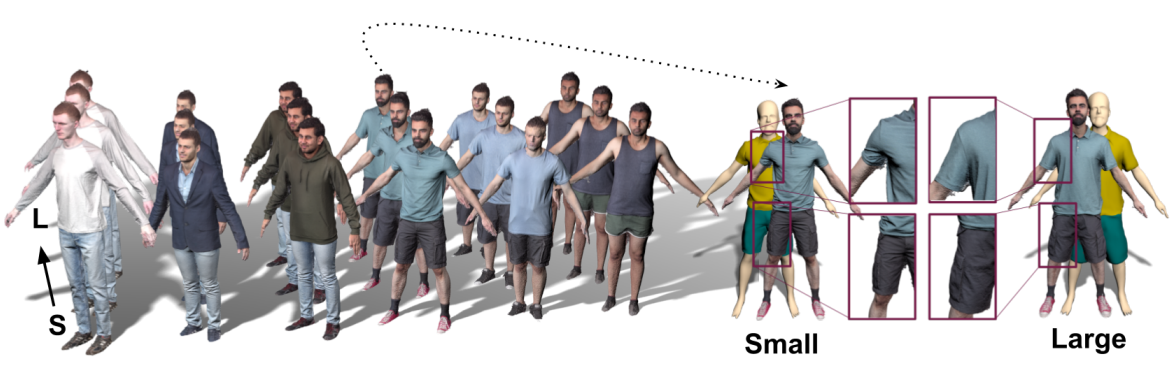
\includegraphics[scale=0.4]{Images/SizerPic/SizerDataset.png}
  \caption{(A sinistra): scansioni 3D di
persone in diversi stili e taglie di abbigliamento. (Destra): maglietta e pantaloncini
pantaloni per taglie piccole e grandi, che sono registrati su modelli comuni.}
  \label{fig:SizerDataset}
\end{figure}

\medskip\medskip\medskip

E’ stato scelto di catturare le mesh dei soggetti in una A-pose in modo tale da avere una vestibilità il più naturale e senza pieghe possibile.
Poiché le scansioni sono state acquisite mediante più di 130 fotocamere e ricostruite con il software \textit{Agisoft’s Metashape}, hanno alta risoluzione e i grafi delle diverse mesh che le rappresentano hanno differenti connessioni, quindi sarebbe difficoltoso utilizzare tale dataset, per questo motivo è stato necessario aggiungere al modello una fase di preprocessing del dataset, registrando le scansioni al modello SMPL.

\medskip\medskip\medskip

SMPL rappresenta il corpo umano come una funzione parametrica di posa e forma.
SMPL+G è una formulazione parametrica che permette di rappresentare corpo e vestiti come mesh separate. Per registrare gli indumenti bisogna per prima cosa segmentare le scansioni in modo da dividere le parti relative al corpo e quelle relative ai vestiti. Per ogni classe di vestiti si ottiene una mesh template definita come un subset del template di SMPL, dove ogni vertice dell’indumento è associato ad un vertice della forma fisica, come offset di quest’ultima.

\medskip

Dunque, il dataset contiene scansioni, scansioni segmentate, registrazioni SMPL+G, classi di indumenti e le taglie come etichette, ed è stato costruito per costruire un modello per l’estrazione di vestiti da una singola mesh (ParserNet) ed un resizing dei vestiti stessi (SizerNet).

\newpage

\begin{figure}[ht!]
  \centering
  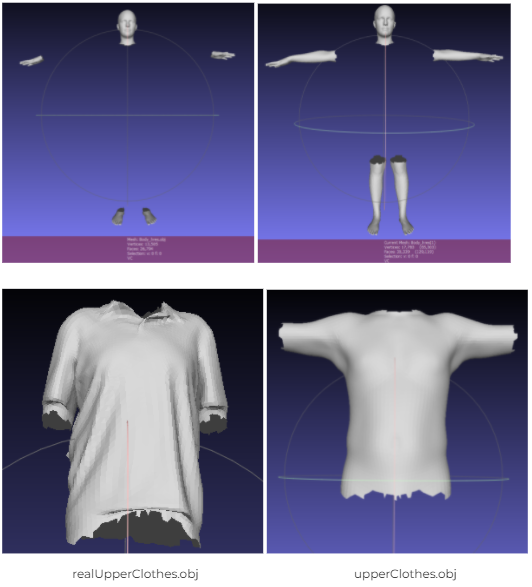
\includegraphics[scale=0.9]{Images/SizerPic/Sizer1.5.png}
    \label{fig:Sizer1.5}
\end{figure}

\medskip

Per ottenere il dataset è necessario andare alla sezione Data del sito \url{http://virtualhumans.mpi-inf.mpg.de/sizer/}.

\medskip

I soggetti delle scansioni di cui è composto il dataset hanno una età compresa tra i 19 e i 37 anni, con due sole eccezioni (51 e 69 anni). Per quel che riguarda l’altezza e il peso dei soggetti scansionati, invece, vi è un range piuttosto vasto, che permette una forte differenziazione dei dati.

\medskip

Il dataset è composto da scansioni di sole A-pose. Tali scansioni sono suddivise per genere e per tipologia di indumento (che può essere a maniche lunghe, maniche corte, pantalone lungo e pantalone corto). Come si può vedere dalle immagini seguenti, sono presenti anche gli oggetti utili a capire quali sezioni del corpo umano escludere dall’estrazione della superficie relativa agli abiti.

\newpage

Poiché il dataset SIZER include registrazioni sul modello SMPL , bisogna scaricare il modello SMPL \url{https://smpl.is.tue.mpg.de/}, che prende in input i parametri di forma e posa e restituisce il volume.

\medskip

\begin{figure}[ht!]
  \centering
  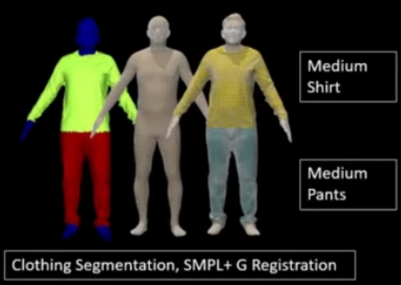
\includegraphics[scale=1]{Images/SizerPic/Sizer2.png}
    \label{fig:Sizer2}
\end{figure}

\paragraph{Preprocessing}
Il dataset SIZER è stato ottenuto tramite una feature extraction effettuata mediante due metodi illustrati di seguito nel dettaglio.

\subsection{Confronto tra SIZER e altri datasets}

Ad oggi, pochi dataset contengono scansioni di modelli tridimensionali relativi a soggetti e vestiti segmentati. Tra questi 3DPeople, Cloth3D consistono di un vasto dataset di rappresentazioni sintetiche di soggetti 3D vestiti. Ma non contengono deformazioni realistiche degli indumenti, come fa invece SIZER. THUman contiene sequenze di persone 3D con relativi abiti in movimento, catturati grazie ad un sensore RGBD (Kinectv2), e ricostruiti utilizzando un fusore volumetrico SDF. Tali scansioni, però, perdono di dettaglio rispetto alle scansioni 3D di SIZER e non vengono fornite le segmentazioni degli indumenti reali. Dyna e D-FAUST, invece, riguardano scansioni 3D ad alta risoluzione di  10 soggetti in movimento con forme differenti; l'unica pecca è che indossano solo vestiti "semplici". BUFF contiene scansioni ad alta risoluzione 3D di 6 soggetti con e senza abiti; neanche questo dataset tuttavia garantisce la segmentazione degli abiti: infatti è stato ideato per addestrare modelli per stimare solo la body shape che si trova al di sotto dei vestiti. 
DeepFashion3D riguarda scansioni di vari tipi di vestiti e potrebbe essere sostituito a SIZER per l'addestramento della rete neurale.








\newpage



\section{Metodo}




\medskip

Siccome queste scansioni sono ad alta risoluzione e rappresentate da mesh con diverse connettività ai grafi sottolineanti (ovvero grafi dove ogni arco direzionato viene sostituito con un vertice privo di direzione) risulta complicato utilizzare tale dataset per qualsiasi modello di apprendimento. Per questo motivo è necessario eseguire un preprocessing registrando grazie all'utilizzo di SMPL.

\medskip

Per migliorare il funzionamento generale del dataset SIZER, vengono implementate le registrazioni SMPL+G.\\
Le scansioni vengono registrate tramite SMPL ampiamente descritto nella prima parte della relazione, realizzando così una corrispondenza tra le scansioni del dataset e SMPL stesso, garantendo un maggior controllo sui parametri di posa e forma tramite sottolineatura fornita sempre da SMPL.


\medskip

Vediamo ora un breve funzionamento di SMPL e SMPL+G specifico a SIZER:

\medskip

SMPL rappresenta il corpo umano come funzione parametrica $M(\cdot)$, di posa $(\theta)$ e forma $(\beta)$.Vengono aggiunti degli offset relativi ai vertici $(D)$ in aggiunta ai modelli delle deformazioni SMPL in grado di gestire capelli, vestiti etc.\\
SMPL applica una forma base del corpo $W(\cdot)$ ad un template preimpostato $T$ posto, appunto, in T-pose.

\medskip

Da qui, W descrive una scala di pesi $B_{p}(\cdot)$ and $B_{s}(\cdot)$, deformazioni dei modelli relativi rispettivamente a posa e forma.

\medskip

\begin{equation*}
\begin{gathered}
M(\boldsymbol{\beta}, \boldsymbol{\theta}, \mathbf{D})=W(T(\boldsymbol{\beta}, \boldsymbol{\theta}, \mathbf{D}), J(\boldsymbol{\beta}), \boldsymbol{\theta}, \mathbf{W}) \\
T(\boldsymbol{\beta}, \boldsymbol{\theta}, \mathbf{D})=\mathbf{T}+B_{s}(\boldsymbol{\beta})+B_{p}(\boldsymbol{\theta})+\mathbf{D}
\end{gathered}
\end{equation*}

\medskip

SMPL+G, invece, è una formulazione parametrica per rappresentare il corpo umano ed i vestiti in mesh separate.\\
Per registrare i vestiti vengono prima segmentate le scansioni relative alle varie parti del corpo.

\medskip

Per ogni classe di indumenti viene ottenuto un template (sottoforma di mesh), definito come un subset del template generato da SMPL, dato da: $T^{g}(\boldsymbol{\beta}, \boldsymbol{\theta}, \boldsymbol{0})=$ $\mathbf{I}^{g} T(\boldsymbol{\beta}, \boldsymbol{\theta}, \mathbf{0})$, dove $\mathbf{I}^{g} \in \mathbb{Z}_{2}^{m_{g} \times n}$ è un indicatore di matrice, con $\mathbf{I}_{i, j}^{g}=1$ se i vertici $i$ dell'abito in questione $g$ $i \in\left\{1 \ldots m_{g}\right\}$ sono associati con la corrispettiva forma del corpo tracciata dai vertici dati dalla scansione $j \in\{1 \ldots n\} . m^{g}$ e $n$ denota il numero di vertici appartenenti al template del vestito e delle mesh SMPL rispettivamente. Similmente viene definita una funzione specifica all'abito $G\left(\boldsymbol{\beta}, \boldsymbol{\theta}, \mathbf{D}^{g}\right)$ usando l'equazione descritta subito sotto, dove $\mathbf{D}^{g}$ sono gli offsets dei vertici ricavati dal template.

\medskip

\begin{equation*}
G\left(\boldsymbol{\beta}, \boldsymbol{\theta}, \mathbf{D}^{g}\right)=W\left(T^{g}\left(\boldsymbol{\beta}, \boldsymbol{\theta}, \mathbf{D}^{g}\right), J(\boldsymbol{\beta}), \boldsymbol{\theta}, \mathbf{W}\right)
\end{equation*}

\medskip

Il dataset preprocessato servirà a costruire il modello ParserNet per l'estrazione dei vestiti dalle singole mesh.

\medskip

\subsection{ParserNet}

\medskip

ParserNet è un metodo per l'estrazione dei vestiti partendo direttamente dalle mesh SMPL. Per fare ciò, è necessario predire i parametri SMPL del corpo sottostante utilizzando una rete per predire posa e forma del corpo umano. Successivamente si applica ParserNet per l'estrazione dei vari livelli di vestiti e di features quali capelli, caratteristiche facciali usate per modellare la body shape sotto i vestiti.

\medskip

\subsubsection{Rete per la predizione di posa e forma}

Per stimare la body shape sotto i vestiti viene inizialmente creato un corpo svestito (tramite SMPL) per uno specifico input dato da una persona vestita fornito tramite mesh ad unico layer $M(\boldsymbol{\beta}, \boldsymbol{\theta}, \mathbf{D})$, prevedendo $\boldsymbol{\theta}, \boldsymbol{\beta}$, usando rispettivamente $f_{w}^{\boldsymbol{\theta}}$ and $f_{w}^{\boldsymbol{\beta}}$. Viene applicato il processo di training $f_{w}^{\theta}$ e $f_{w}^{\boldsymbol{\beta}}$ con una perdita $L_{2}$ sui parametri e una perdita per-vertex tra la mesh di input e il corpo predetto da SMPL. 

\medskip

\begin{equation*}
\begin{gathered}
\mathcal{L}_{\boldsymbol{\theta}}=w_{\text {pose }}\|\hat{\boldsymbol{\theta}}-\boldsymbol{\theta}\|_{2}^{2}+w_{v}\|M(\boldsymbol{\beta}, \hat{\boldsymbol{\theta}}, \mathbf{0})-M(\boldsymbol{\beta}, \boldsymbol{\theta}, \mathbf{D})\| \\
\mathcal{L}_{\boldsymbol{\beta}}=w_{\text {shape }} \sum_{i=1}^{10} \sigma_{i}\left(\hat{\boldsymbol{\beta}}_{i}-\boldsymbol{\beta}_{i}\right)^{2}+w_{v}\|M(\hat{\boldsymbol{\beta}}, \boldsymbol{\theta}, \mathbf{0})-M(\boldsymbol{\beta}, \boldsymbol{\theta}, \mathbf{D})\|
\end{gathered}
\end{equation*}

\medskip

Siccome i parametri $\boldsymbol{\theta}, \boldsymbol{\beta}$, relativi al corpo di riferimento possono essere imprecisi, viene aggiunta una perdita relativa ai vertici addizionale tra la mesh data input $M(\boldsymbol{\beta}, \boldsymbol{\theta}, \mathbf{D})$ ed i vertici del corpo predetto $M(\hat{\boldsymbol{\theta}}, \hat{\boldsymbol{\beta}}, \mathbf{0})$ in modo tale da ottenere un corpo svestito il più simile possibile a quello della mesh data in input.

\medskip

Facendo il training di $f_{w}^{\theta}$ e $f_{w}^{\beta}$\ separatamente si osservano risultati più stabili, usando come riferimenti $\beta$ e $\theta$.
Poichè le componenti di $\beta$ in SMPL sono normalizzate (ovvero $\sigma=1$), vengono denormalizzate scalando le loro corrispettive deviazioni standard $\left[\sigma_{1}, \sigma_{2}, \ldots, \sigma_{10}\right]$ come dimostrato nell'equazione sottostante.

\medskip

\begin{equation*}
\begin{gathered}
\mathcal{L}_{\boldsymbol{\theta}}=w_{\text {pose }}\|\hat{\boldsymbol{\theta}}-\boldsymbol{\theta}\|_{2}^{2}+w_{v}\|M(\boldsymbol{\beta}, \hat{\boldsymbol{\theta}}, \mathbf{0})-M(\boldsymbol{\beta}, \boldsymbol{\theta}, \mathbf{D})\| \\
\mathcal{L}_{\boldsymbol{\beta}}=w_{\text {shape }} \sum_{i=1}^{10} \sigma_{i}\left(\hat{\boldsymbol{\beta}}_{i}-\boldsymbol{\beta}_{i}\right)^{2}+w_{v}\|M(\hat{\boldsymbol{\beta}}, \boldsymbol{\theta}, \boldsymbol{0})-M(\boldsymbol{\beta}, \boldsymbol{\theta}, \mathbf{D})\|
\end{gathered}
\end{equation*}

\medskip

Qui, $w_{\text {pose }}, w_{\text {shape }}$ e $w_{v}$ sono pesi relativi alla perdita su posa, forma e superficie SMPL predetta. $(\hat{\boldsymbol{\theta}}, \hat{\boldsymbol{\beta}})$ denotano i parametri predetti. Il risultato sarà una body shape svestita lineare.


Here, $w_{\text {pose }}, w_{\text {shape }}$ and $w_{v}$ are weights for the loss on pose, shape and predicted SMPL surface. $(\hat{\boldsymbol{\theta}}, \hat{\boldsymbol{\beta}})$ denote predicted parameters. The output is a smooth (SMPL model) body shape under clothing.

\subsection{Analisi dei vestiti}

\medskip

L'analisi dei vestiti ottenuti tramite una singola mesh $(M)$ può essere ottenuta segmentando la mesh stessa in vestiti separati per ogni classe di appartenenza $\left(\mathbf{G}_{\mathrm{seg}}^{g, k}\right)$, che si traduce nella connettività di diversi grafo sottostante $\left(\mathcal{G}_{\text {seg }}^{g, k}=\left(\mathbf{G}_{\mathrm{seg}}^{g, k}, \mathbf{E}_{\mathrm{seg}}^{g, k}\right)\right)$ attraverso tutte le istanze (k) di un vestito appartenente alla classe g come si può vedere nella figura sottostante. Siccome tale procedimento rende difficile la generalizzazione del dataset in qualsiasi modello di apprendimento, pertanto viene proposto di effettuare il parsing dei vestiti deformando i vertici dei vestiti relativi al template T: $T^{g}(\boldsymbol{\beta}, \boldsymbol{\theta}, \mathbf{0})$ con connettività fissata $\mathbf{E}^{g}$, ottenendo i vertici $\mathbf{G}^{g, k} \in \mathcal{G}^{g, k}$, dove $\mathcal{G}^{g, k}=\left(\mathbf{G}^{g, k}, \mathbf{E}^{g}\right)$ sono visibili nella parte centrale della figura sottostante.

\medskip

Si procede a prevedere i vertici deformati $\mathbf{G}^{g}$ come una conbinazione convessa dei vertici presi dalla mesh di input iniziale $\mathbf{M}=M(\boldsymbol{\beta}, \boldsymbol{\theta}, \mathbf{D})$ utilizzando una matrice a regressione sparsa $\mathbf{W}^{g}$, in modo che risulti $\mathbf{G}^{g}=\mathbf{W}^{g} \mathbf{M}$. Specificatamente, ParserNet predice tale matrice sparsa $\left(\mathbf{W}^{g}\right)$ come una funzione di features di mesh presa in input (vertici e normali) e un insieme di neighbor per ogni vertice i di una classe di vestiti g.

\medskip

$\mathbf{G}_{i}=\sum_{j \in \mathcal{N}_{i}} \mathbf{W}_{i j} \mathbf{M}_{j}$

\medskip

\begin{figure}[ht!]
  \centering
  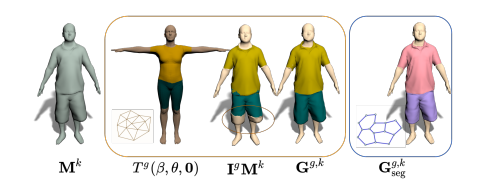
\includegraphics[scale=1]{Images/SizerPic/ParserNet.png}
  \caption{Da sinistra a destra: In input una singola mesh $\left(\mathbf{M}^{k}\right)$, il template dell'abito $\left(T^{g}(\boldsymbol{\beta}, \boldsymbol{\theta}, \mathbf{0})=\right.$ $\left.\mathbf{I}^{g} T(\boldsymbol{\beta}, \boldsymbol{\theta}, \mathbf{0})\right)$, estrazione della mesh del vestito usando $\mathbf{G}^{g, k}=\mathbf{I}^{g} \mathbf{M}^{k}$, mesh multilivello $\left(\mathbf{G}^{g, k}\right)$ registrata a SMPL+G, tutto questo con classi di vestiti munite di specifiche connessioni tra vertici $\mathbf{E}^{g}$, e scansioni segmentate $\mathbf{G}_{\mathrm{seg}}^{g, k}$ con specifiche istanze di connettività tra vertici $\mathbf{E}_{\mathrm{seg}}^{g, k}$.}
  \label{fig:ParserNet}
\end{figure}

\medskip

\subsection{Analisi della body shape svestita}

\medskip

Ai fini di generare una dettagliata body shape svestita, viene prima creata una mesh del corpo lineare, grazie all'utilizzo dei parametri SMPL $\boldsymbol{\theta}$ e $\boldsymbol{\beta}$ ricavati da $f_{w}^{\boldsymbol{\theta}}, f_{w}^{\boldsymbol{\beta}}$. Utilizzando la formulazione di combinazione convessa citata sopra, Body ParserNet trasferisce i vertici della pelle visibile dalla mesh data in input a quella lineare creata, ottenendo così le caratteristiche facciali e relative ai capelli.Successivamente viene scomposta la mesh di input in magliette, pantaloni e forma del corpo svestita utilizzando le 3 sottoreti di ParserNet $\left(f_{w}^{U}, f_{w}^{L}, f_{w}^{B}\right)$ mostrate in figura 1.3.

\medskip

\subsection{Funzione di Loss}

\medskip

La rete ParserNet viene addestrata tramite la funzione di Loss sotto descritta: 
\medskip

\begin{equation*}
\begin{gathered}
\mathcal{L}_{\text {parser }}=w_{3 \mathrm{D}} \mathcal{L}_{3 \mathrm{D}}+w_{\text {norm }} \mathcal{L}_{\text {norm }}+w_{\text {lap }} \mathcal{L}_{\text {lap }}+w_{\text {interp }} \mathcal{L}_{\text {interp }}+w_{\mathrm{w}} \mathcal{L}_{\mathrm{w}} \\
\mathcal{L}_{\text {sizer }}=w_{3 \mathrm{D}} \mathcal{L}_{3 \mathrm{D}}+w_{\text {norm }} \mathcal{L}_{\text {norm }}+w_{\text {lap }} \mathcal{L}_{\text {lap }}+w_{\text {interp }} \mathcal{L}_{\text {interp }}
\end{gathered}
\end{equation*}

\medskip

dove $w_{3 \mathrm{D}}, w_{\text {norm }}, w_{\text {lap }}, w_{\text {interp }}$ and $w_{\mathrm{w}}$ sono i pesi relativi ai vertici di Loss, normali, Laplaciani, di interpenetrazione e di termini di regolarizzazione dei pesi.

\subsubsection{3D Vertex Loss per vestiti}

\medskip

Viene definito $\mathcal{L}_{3 D}$ come una Loss nello spazio $L_{1}$ tra vertici predetti ed effettivi.

\medskip

$$
\mathcal{L}_{3 \mathrm{D}}=\left\|\mathbf{G}_{\mathrm{P}}-\mathbf{G}_{\mathrm{GT}}\right\|_{1} .
$$

\medskip

\subsubsection{3D Vertex Loss corpi svestiti}

Per addestrare $f_{w}^{B}$ (ParserNet specifica per il corpo), viene utilizzata la mesh di input relativa alla pelle come supervisione per prevedere i dettagli personali del soggetto. Si definisce un termine di loss pesato (tramite la distanza geodetica) specifico per ogni classe di vestiti. 

\medskip

$$
\mathcal{L}_{3 \mathrm{D}}^{\text {body }}=\left\|\boldsymbol{w}_{\text {geo }}^{T} \cdot \operatorname{abs}_{i j}\left(\mathbf{G}_{\mathrm{P}}^{s}-\mathbf{I}^{s} \mathbf{M}\right)\right\|_{1}
$$

\medskip

dove $\mathbf{I}^{s}$ è la matrice di indicatori per la specifica regione di pelle e $\boldsymbol{w}_{\text {geo }}$ è un vettore contenente il sigmoide del termine di loss specifico ottenuto tramite distanza geodetica dai vertici appartenenti alla regione relativa alla pelle e non. Il termine di Loss è elevato quando la predizione è molto diversa dalla mesh originale di input $\mathbf{M}$ relativa alle porzioni di pelle visibili, e bassa per quanto riguarda le regioni relative agli indumenti, con una transizione lineare regolata dal termine geodetico. Nella formulazione citata sopra, il termine $\operatorname{abs}_{i j}(\cdot)$ rappresenta un operatore di valore assoluto.  
\medskip

\subsubsection{Normal Loss}

\medskip

Viene definito $\mathcal{L}_{\text {norm }}$ come la differenza in angolo tra la faccia normalizzata reale $\left(\mathbf{N}_{G T}^{i}\right)$ e quella predetta $\left(\mathbf{N}_{P}^{i}\right)$.

\medskip

\subsubsection{Termine di smoothness Laplaciano}

\medskip

Si definisce $\mathbf{L}^{g} \in$ $\mathbb{R}^{m_{g} \times m_{g}}$ come grafo Laplaciano relativo alla mesh dell'abito $\mathbf{G}_{\mathrm{GT}}$, e $\boldsymbol{\Delta}_{\text {init }}=$ $\mathbf{L}^{g} \mathbf{G}_{\mathrm{GT}} \in \mathbb{R}^{m_{g} \times 3}$ come le coordinate differenziali di $\mathbf{G}_{\mathrm{GT}}$, successivamente di computa il termine di smoothness Laplaciano per una predetta mesh $\mathbf{G}_{\mathrm{P}}$ come 

\medskip

$$
\mathcal{L}_{\text {lap }}=\left\|\boldsymbol{\Delta}_{\text {init }}-\mathbf{L}^{g} \mathbf{G}_{\mathrm{P}}\right\|_{2} .
$$

\medskip

\subsubsection{Interpenetration loss}

\medskip

Siccome minimizzare la perdita specifica dei vertici non garantisce che l'indumento predetto sia esterno alla superficie del corpo, viene utilizzato il termine di Interpenetration loss: 

$$
\mathcal{L}_{\text {interp }}=\sum_{(i, j) \in \mathcal{C}\left(\mathbf{B}, \mathbf{G}_{\mathrm{P}}\right)} \mathbb{1}_{d\left(\mathbf{G}_{\mathrm{P}, j}, \boldsymbol{G}_{\mathrm{GT}, j}\right)<d_{\text {tol }}} \operatorname{ReLU}\left(-\mathbf{N}_{i}\left(\mathbf{G}_{\mathrm{P}, j}-\mathbf{B}_{i}\right)\right) / m_{g},
$$

\medskip

Per ogni vertice $\mathbf{G}_{\mathbf{P}, j}$ viene trovato quello più vicino all'interno della body shape svestita predetta  $\mathbf{B}_{i}$ e viene definita una corrispondenza corpo-vestito $\mathcal{C}\left(\mathbf{B}, \mathbf{G}_{\mathrm{P}}\right)$. Se il vertice relativo all'indumento $\mathbf{G}_{\mathrm{P}, j}$ si trova all'interno della superficie del corpo, il modello viene penalizzato mediante la formula sopra descritta.

da notare che $\mathbb{1}_{d\left(\mathbf{G}_{\mathrm{P}, j}, \boldsymbol{G}_{\mathrm{GT}, j}\right)<d_{t o l}}$ attiva il termine di loss solo quando la distanza tra i vertici della mesh del vestito predetta ed i vertici della mesh reale è piccola, ad esempio: $<d_{\text {tol }}$.





\medskip

\subsubsection{Regolarizzazione dei pesi}

\medskip

Per mantenere i dettagli più particolari e fini mentre viene divisa la mesh in input si vuole che i pesi della rete siano sparsi e racchiusi all'interno di un unico cluster. Conseguentemente viene aggiunto un regolarizzatore che penalizza valori elevati per $\mathbf{W}_{i j}$ se la distanza tra $\mathbf{M}_{j}$ ed il vertice $\mathbf{M}_{k}$ (con peso maggiore $k=\arg \max _{j} \mathbf{W}_{i j}$) è grande. Viene definito $d(\cdot, \cdot)$ come distanza Euclidea tra i vertici, allora il regolarizzatore equivale a:

\medskip

$$
\mathcal{L}_{w}=\sum_{i=1}^{m_{g}} \sum_{j \in \mathcal{N}_{i}} \mathbf{W}_{i j} d\left(\mathbf{M}_{k}, \mathbf{M}_{j}\right), k=\arg \max _{j} \mathbf{W}_{i j}
$$

\subsection{Cenno sulle reti neurali utilizzate}

\medskip

Vengono implementate $f_{w}^{\boldsymbol{\theta}}$ e $f_{w}^{\boldsymbol{\beta}}$: reti con con due livelli completamente connessi ed un livello di output lineare. Successivamente si implementa ParserNet $f_{w}^{U}, f_{w}^{L}, f_{w}^{B}$ con 3 livelli completamente connessi. Nello specifico caso di SIZER sono stati utilizzati per gli esperimenti cluster $\left(\mathcal{N}_{i}\right)$ di dimensione 50. 
Inizialmente viene addestrata la rete con classi di vestiti che condividono lo stesso template e successivamente si adattano separatamente per ogni classe $g$.
Per velocizzare il processo di addestramento di ParserNet, si addestra la rete a prevedere $\mathbf{W}^{g}=\mathbf{I}^{g}$, dove $\mathbf{I}^{g}$ riguarda la matrice di indicatori per la classe di vestito $g$.
Grazie a ciò, si inizializza il processo per il quale la rete suddivide il vestito tagliando parte della mesh di input basata sulla matrice di indicatori per ogni vestito.

\medskip

Per la rete di predizione di posa e form, ParserNet usa una dimensione di batch = 8 e una curva di apprendimento di $0.0001$.






\newpage

\section{Codice}

\medskip

Per utilizzare il codice (\url{https://github.com/garvita-tiwari/sizer}) sono necessari come prerequisiti le librerie mesh e kaolin.
In caso di dubbi sui passaggi da seguire, di seguito vengono riportate le istruzioni in maniera semplificata.

\medskip

Di seguito viene illustrata una guida alle installazioni a seconda del sistema operativo di cui si è in possesso.

\medskip

\section{Linux}

\medskip

I comandi mostrati successivamente sono stati testati su una distribuzione Ubuntu 20.04, con la versione di Python 3.6.8.

\medskip

Per prima cosa, bisogna installare le librerie di Boost (\url{https://www.boost.org/users/history/version_1_77_0.html}), in quanto serviranno per l’utilizzo di Psbody-mesh.

\medskip

\begin{itemize}
\item \textit{\$ sudo apt-get install libboost-dev
\item \$ sudo apt install python3.8-venv
\item \$ (opzionale) $>$ mkdir python-venvs
\item \$ (opzionale) $>$ cd python-venvs
\item \$ python3 -m venv --copies <venv\_name>
\item \$ source <venv\_name>/bin/activate
\item \$ mkdir workspace
\item \$ cd workspace/}
\end{itemize}







\medskip

La directory workspace è stata creata per far sì che tutte le librerie che si andranno ad installare si trovino in un unico ambiente di lavoro; durante la loro installazione, quindi, è importante trovarsi nella cartella principale del workspace.


\medskip

\subsubsection{Psbody-mesh}

Questo pacchetto contiene le principali funzioni di manipolazione e visualizzazione di mesh. Richiede Python3.5$+$ e le librerie di Boost.

\medskip





\begin{itemize}
\item \textit{\$ sudo apt install git
\item \$ git clone https://github.com/MPI-IS/mesh
\item \$ cd mesh}
\end{itemize}


\medskip
A questo punto, nel caso in cui la variabile BOOST\_INCLUDE\_DIRS non sia settata, 
bisogna eseguire il seguente comando: 

\code{\$ BOOST\_INCLUDE\_DIRS=/path/to/boost/include make all}




\medskip

Ciò può essere verificato mediante 

\medskip



\code{\$ echo BOOST\_INCLUDE\_IRS.}



\medskip\medskip\medskip

Per ottenere il percorso in cui si trova boost:




\code{\$ whereis boost}



\medskip

Se la compilazione dà errore su Python.h, può significare che dall’installazione di Python manchino i file sorgenti, quindi è necessario cercare il nome della libreria installata e completare l’installazione.

\medskip

\begin{itemize}
\item \textit{\$ sudo apt search libpython
\item \$ sudo apt install libpython3.8-dev}
\end{itemize}




Dopodiché ripetere

\medskip



\code{\$ BOOST\_INCLUDE\_DIRS=/path/to/boost/include make all}



\medskip

A questo punto, l’installazione del pacchetto psbody-mesh è completata e la si può testare mediante \$ make tests.

\medskip

Per ottenere la documentazione e visualizzarla:

\begin{itemize}
\item \textit{\$ make documentation
\item \$ firefox /path/to/mesh/doc/build/html/index.html}
\end{itemize}




\medskip

\subsubsection{Kaolin}

La libreria di NVIDIA Kaolin fa parte di una suite di strumenti per la ricerca sul deep learning 3D. Fornisce una API di PyTorch utile per lavorare con una varietà di rappresentazioni 3D, comprende una raccolta sempre crescente di operazioni ottimizzate per la GPU come rendering differenziabile modulare, conversioni veloci tra rappresentazioni, caricamento dei dati, checkpoint 3D e altro.


\medskip

Requisiti:

\begin{itemize}
\item \textit{Python $>$= 3.6
\item CUDA $>$= 10.0 (con ‘nvcc’ installato)
\item torch $>$= 1.5, $<$= 1.7.1
\item cython == 0.29.20
\item scipy $>$= 1.2.0
\item Pillow $>$= 8.0.0
\item usd-core $>$= 20.11 (opzionale, richiesto per le librerie di Python USD (Universal Scene Description).}

\end{itemize}

\newpage


\subsubsection{CUDA}

\medskip



\code{\$ sudo apt install nvidia-cuda-toolkit}



\medskip

\begin{figure}[ht!]
  \centering
  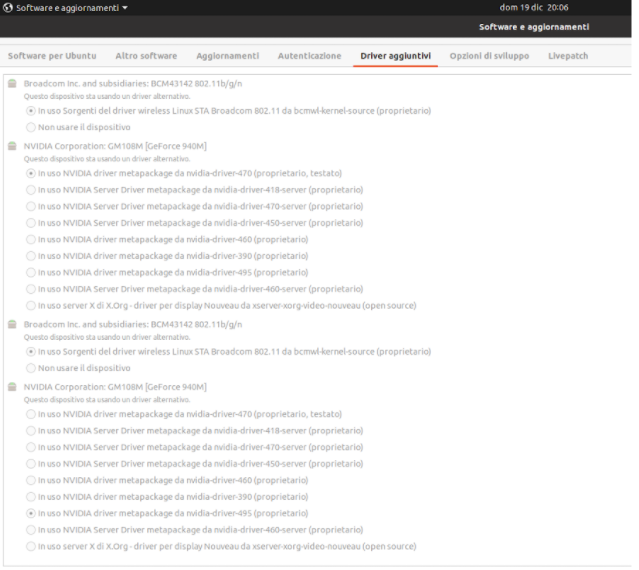
\includegraphics[scale=0.8]{Images/SizerPic/Sizer9.png}
    \label{fig:Sizer9}
\end{figure}

\medskip



\code{\$ sudo apt install cuda}



\medskip

Per assicurarsi di utilizzare la scheda grafica NVIDIA:

\medskip

\code{\$ sudo prime-select intel}

\code{\$ sudo prime-select nvidia}


\medskip

Per avere informazioni sulla scheda grafica:

\medskip



\code{\$ nvidia-smi}



\subsubsection{Installazione di Kaolin}

\medskip

\begin{itemize}
\item \textit{\$ git clone --recursive 
\item \$ cd kaolin
\item \$ git checkout v0.9.0
\item \$ python setup.py develop}
\end{itemize}




website: \url{https://github.com/NVIDIAGameWorks/kaolin}

\medskip

Se durante la fase di setup non dovessero essere trovati torch e/o cython, installarli utilizzando i seguenti comandi:

\medskip

\begin{itemize}
\item \$ pip install torch torchvision
\item \$ pip install Cython
\end{itemize}



\medskip



\code{nvcc warning :} The 'compute\_35', 'compute\_37', 'compute\_50', 'sm\_35', 
'sm\_37' and 'sm\_50' architectures are deprecated, 
and may be removed in a future release (Use -Wno-deprecated-gpu-targets to suppress warning).



\medskip

Questo significa che, per la versione di kaolin 0.9, la GPU risulta deprecata.

\medskip

L’installazione di kaolin v0.1, invece, dà errore perché manca la libreria pptk, la cui wheel non è più reperibile e anche la compilazione dai file sorgenti causa problemi.

\medskip

Kaolin vuole gcc e g$++$ 8 e vuole che la versione di CUDA sia uguale a quella usata da Pytorch, che nell’ultima versione corrisponde a CUDA 10.2.
CUDA 10.2 richiede  gcc e g$++$ 9.

\medskip

Bisogna trovare una versione di PyTorch che usi CUDA 9 (PyTorch 1.2 dovrebbe essere compatibile con CUDA 9), potrebbero tuttavia esserci delle interferenze di compatibilità con gcc v8.

\medskip

Per verificare la possibilità di importare kaolin, si può testare la sua installazione nel seguente modo:

\medskip



\code{\$ python -c "import kaolin; print(kaolin.\_\_version\_\_)"}



\newpage

\subsection{Sizer}

\medskip\medskip\medskip



\code{\$ git clone --recursive https://github.com/garvita-tiwari/sizer}




\medskip\medskip\medskip

Poiché il dataset SIZER include registrazioni sul modello SMPL, bisogna scaricare il modello SMPL \url{https://smpl.is.tue.mpg.de/} e salvarlo nella cartella di sizer training\_{}data.

\medskip\medskip\medskip

\begin{figure}[ht!]
  \centering
  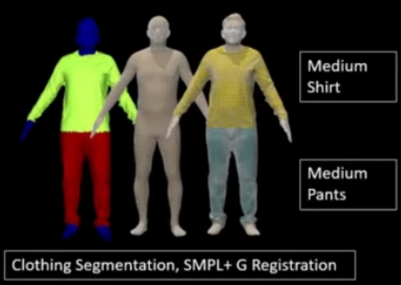
\includegraphics[scale=1]{Images/SizerPic/Sizer2.png}
    \label{fig:Sizer2}
\end{figure}

\medskip\medskip\medskip

Settare

\medskip\medskip\medskip

\code{DATA\_DIR='<downloaded dataset path>/training\_data' in utils/global\_var.py}



\medskip

A questo punto è possibile fare la validazione di ParserNet:




\code{\$ python trainer/parsernet\_eval.py --log\_dir <log\_dir\_path> \-}



\medskip

Si consiglia di salvare i file di log in una cartella dedicata all’interno di quella del progetto Sizer, invece che in trainer, in modo da non contaminare la cartella contenente i file di addestramento.
Se i moduli tensorboardX e ipdb non dovessero essere trovati, procedere alla loro installazione mediante i seguenti comandi:

\medskip

\begin{itemize}
\item \textit{\$ pip install tensorboardX
\item \$ pip install ipdb}
\end{itemize}




\medskip

In caso di errori sugli import, come ad esempio ImportError: cannot import name 'TriangleMesh' from 'kaolin.rep', si consiglia di effettuare il downgrade di torch alla versione 1.4, con la quale il codice sizer è stato testato, oppure, se il problema persiste, passare alla versione 0.1 di kaolin se non è già stato fatto, in quanto dalla versione 0.9 di Kaolin TriangleMesh non esiste più.

\medskip

\begin{itemize}
\item \textit{/kaolin\$ git checkout v0.1
\item /kaolin\$ python setup.py develop}
\end{itemize}



\begin{enumerate}
\item \url{https://githubmemory.com/repo/NVIDIAGameWorks/kaolin/issues/414} 
\item \url{https://github.com/pytorch/pytorch/issues/38090}
\item \url{https://github.com/garvita-tiwari/sizer}
\end{enumerate}




\newpage

\section{Windows}

\medskip

Create a dedicated Python virtual environment and activate it:

\medskip

\code{$>$ conda create -n my\_env (garments)}

\medskip

\code{$>$ conda activate my\_env}



\medskip

Per prima cosa bisogna installare le librerie di Boost.
Si può decidere di seguire le linee guida nel file README \url{https://www.boost.org/users/history/version_1_77_0.html} oppure installarlo da github \url{https://gist.github.com/sim642/29caef3cc8afaa273ce6}

\medskip

Unzip il file boost e seguire le istruzioni presenti in index.html.

\medskip

\subsection{Boost}

\medskip


Leggere il file "Install" per maggiori informazioni.

\medskip

\begin{itemize}
\item Andare nella directory tools -build-.
\item Eseguire bootstrap.bat (sul prompt dei comandi scrivere:  \\ \code{start bootstrap.bat}
\item Eseguire b2install \textit{--prefix=PREFIX} dove PREFIX è la directory dove si vuole installare Boost.Build\\ \code{start b2 install --prefix=.-build}
\end{itemize}


\medskip

Cerca il toolset adatto al compilatore che vuoi utilizzare su Pycharm dalla tabella nel seguente link: (una lista aggiornata è disponibile anche nella documentazione di \textit{Boost.Build})

\medskip

\url{https://www.boost.org/doc/libs/1_77_0/tools/build/doc/html/index.html#bbv2.reference.tools}

\medskip

\subsection{Librerie Boost per GCC}

\medskip

Guida per installare le librerie di Boost per GCC (MinGW): \\
\url{https://gist.github.com/sim642/29caef3cc8afaa273ce6}

\medskip

\subsection{Psbody-mesh}

\medskip

A questo punto, bisogna compilare ed installare il pacchetto Psbody-mesh usando il Makefile:

\medskip

\begin{itemize}
\item cd .path/to/mesh-master
\item make all
\end{itemize}

\medskip

In caso di errori quali

\code{pip uninstall spyder} 

\medskip

\code{pip 10 no longer uninstalls distutils packages}

\medskip 

fare il downgrade a pip 8.1.1.:

\medskip

\code{sudo -H pip3 install pip==8.1.1}




\medskip

Psbody-mesh contiene le principali funzioni di manipolazione e visualizzazione di mesh. Richiede Python3.5$+$ e le librerie di Boost installate seguendo il paragrafo precedente.

\newpage

\subsection{Kaolin}

\medskip

E’ necessaria l’installazione della libreria Kaolin, che può essere effettuata seguendo le linee guida del sito ufficiale: 

\medskip

\url{https://kaolin.readthedocs.io/en/latest/notes/installation.html}

\medskip

La libreria di NVIDIA Kaolin fa parte di una suite di strumenti per la ricerca sul deep learning 3D. Fornisce una API di PyTorch utile per lavorare con una varietà di rappresentazioni 3D, comprende una raccolta sempre crescente di operazioni ottimizzate per la GPU come rendering differenziabile modulare, conversioni veloci tra rappresentazioni, caricamento dei dati, checkpoint 3D e altro.

\medskip

Requisiti:

\begin{itemize}
\item \textit{Python $>$= 3.6
\item CUDA $>$= 10.0 (con nvcc installato)
\item torch $>$= 1.5, $<$= 1.7.1
\item cython == 0.29.20
\item scipy $>$= 1.2.0
\item Pillow $>$= 8.0.0
\item usd-core $>$= 20.11 (opzionale, richiesto per le librerie di Python USD) (Universal Scene Description).}
\end{itemize}







\medskip

E’ possibile eseguire il file di setup di kaolin tramite il terminale di pycharm, all’interno del progetto:
python setup.py install

\medskip



\subsection{Sizer}

\medskip

Scaricare il dataset dalla sezione Data della pagina web di SIZER (\url{http://virtualhumans.mpi-inf.mpg.de/sizer/}), recuperarne il percorso e seguire le istruzioni del README di github (\url{https://github.com/garvita-tiwari/sizer}).



\medskip

\subsection{Installazione dei pacchetti}

\medskip

Per prima cosa è necessario assicurarsi che il pacchetto pip per python 3 sia installato correttamente.

\medskip

In caso contrario, sarà sufficiente eseguire la seguente linea di codice sul terminare direttamente offertoci da pycharm



\code{py -m ensurepip --default-pip}



I pacchetti richiesti dal modello sono 131, facilmente reperibili dal file requirements.txt presente all'interno del github di SIZER. 

\medskip

\url{https://github.com/garvita-tiwari/sizer/blob/master/requirements.txt}

\medskip

Per scaricare le librerie richieste dal file .txt è sufficiente spostarsi, tramite l'utilizzo della shell di python, nella cartella contenente il file requirements.txt ed eseguire il seguente comando:

\medskip

\code{pip install -r requirements.txt}

\medskip

Tuttavia il nome "completo" dei pacchetti inseriti nel documento di testo requirements.txt non corrisponde sempre alla versione richiesta da SIZER.
Per ovviare a questo problema è necessario installare manualmente ogni singolo pacchetto.


\medskip

La maggior parte dei pacchetti è facilmente installabile su pycharm eseguendo il comando pip install [nome pacchetto]

\medskip

Tra questi pacchetti, alcuni necessitano il supporto del terminale di anaconda per essere installati.
Di seguito vengono specificati più comandi d'istallazione per ogni singolo pacchetto in quanto diverse versioni di sistema operativo richiedono diversi comandi compatibili con i rispettivi registri.

\newpage

\begin{table}
\begin{tabular}{ |p{8cm}||p{8cm}|  }




\multicolumn{2}{|c|}{Package List (Windows or Linux)} \\


\textbf{Nome e versione del pacchetto}& \textbf{Comandi per anaconda}\\


libwebp==1.2.0=h89dd481\_0&conda install libwebp==1.2.0  \\



sqlite==3.36.0=hc218d9a\_0&conda install sqlite==3.36.0\\



  sqlite==3.36.0=hc218d9a\_0&	conda install sqlite==3.36.0\\


libwebp-base==1.2.0=h27cfd23\_0&conda install libwebp-base==1.2.0\\


  xz==5.2.5=h7b6447c\_0&	conda install xz==5.2.5\\


  yaml==0.2.5=h516909a\_0&	conda install yaml==0.2.5\\


  pexpect==4.8.0=pypi\_0&	conda install pexpect==4.8.0\\



  jpeg==9d=h7f8727e\_0&	conda install jpeg==9d\\



  numpy==1.21.2=py38h20f2e39\_0&	conda install numpy==1.21.2\\




  giflib==5.2.1=h7b6447c\_0&conda install giflib==5.2.1\\



  libuv==1.40.0=h7b6447c\_0&	conda install libuv==1.40.0\\




  libtiff==4.2.0=h85742a9\_0&	conda install libtiff==4.2.0\\



  mkl\_fft==1.3.1=py38hd3c417c\_0&	conda install mkl\_fft==1.3.1\\



  lcms2==2.12=h3be6417\_0&	conda install lcms2==2.12\\



  mkl\_random==1.2.2=py38h51133e4\_0&	conda install mkl\_random==1.2.2\\



  mkl-service==2.4.0=py38h7f8727e\_0&	conda install mkl-service==2.4.0\\



  cudatoolkit==10.2.89=hfd86e86\_1&	conda install cudatoolkit==10.2.89\\



  scikit-image==0.18.3=pypi\_0&	conda install scikit-image==0.18.3\\



  tk==8.6.11=h1ccaba5\_0&	conda install tk==8.6.11\\



  numpy-base==1.21.2=py38h79a1101\_0&	conda install numpy-base==1.21.2\\



  lz4-c==1.9.3=h295c915\_1&	conda install lz4-c==1.9.3\\




   zstd==1.4.9=haebb681\_0&	conda install zstd==1.4.9\\



   libpng==1.6.37=hbc83047\_0&	conda install libpng==1.6.37\\



   openssl==1.1.1l=h7f8727e\_0&	conda install openssl==1.1.1l\\



 torchvision==0.8.2=cpu\_py38ha229d99\_0&	conda install -c pytorch-lts torchvision\\




  cachetools==4.2.4=pypi\_0&	conda install -c quantopian cachetools\\



  pytorch==1.7.1=py3.8\_cuda10.2.89\_cudnn7.6.5\_0&	conda install -c fastchan pytorch\\


libffi==3.3=he6710b0\_2&conda install -c conda-forge libffi 

conda install -c conda-forge/label/gcc7 libffi 
conda install -c conda-forge/label/broken libffi 
conda install -c conda-forge/label/cf201901 libffi 
conda install -c conda-forge/label/cf202003 libffi\\

  liblapack==3.9.0=12\_linux64\_mkl&	conda install -c conda-forge liblapack  	conda install -c conda-forge/label/broken liblapack 	conda install -c conda-forge/label/cf202003 liblapack\\


  freetype==2.11.0=h70c0345\_0&	conda install -c conda-forge freetype  	conda install -c conda-forge/label/gcc7 freetype 	conda install -c conda-forge/label/cf201901 freetype 	conda install -c conda-forge/label/cf202003 freetype\\


  Shapely-1.8.0&	conda install -c conda-forge shapely 	conda install -c conda-forge/label/gcc7 shapely 	conda install -c conda-forge/label/cf201901 shapely 	conda install -c conda-forge/label/cf202003 shapely 	conda install -c conda-forge/label/shapely\_dev shapely\\




  igl==2.2.1=py38h52fb889\_1&	conda install -c conda-forge igl  	conda install -c conda-forge/label/cf202003 igl\\


  ca-certificates==2021.10.8=ha878542\_0&	conda install -c conda-forge ca-certificates  	conda install -c conda-forge/label/gcc7 ca-certificates  	conda install -c conda-forge/label/broken ca-certificates  	conda install -c conda-forge/label/cf201901 ca-certificates 	conda install -c conda-forge/label/cf202003 ca-certificates\\



\end{tabular}
\end{table}

\newpage

Per quanto riguarda i seguenti pacchetti è necessariamente richiesto Linux come sistema operativo.

\medskip
\begin{table}
\begin{tabular}{ |p{8cm}||p{8cm}|}

\multicolumn{2}{|c|}{Package List (Linux only)} \\


Nome e versione del pacchetto& comandi per anaconda\\ \hline


\multirow{3}{*}{libgomp==9.3.0=h5101ec6\_17}   &	conda install -c conda-forge libgomp \\
& conda install -c conda-forge/label/broken libgomp \\
& conda install -c conda-forge/label/cf202003 libgomp\\ \hline



  libstdcxx-ng==9.3.0=hd4cf53a\_17  &	conda install -c conda-forge libstdcxx-ng conda install -c conda-forge/label/gcc7 libstdcxx-ng  conda install -c conda-forge/label/broken libstdcxx-ng  conda install -c conda-forge/label/cf201901 libstdcxx-ng 	conda install -c conda-forge/label/cf202003 libstdcxx-ng\\ \hline



  ld\_impl\_linux-64==2.35.1=h7274673\_9  &	conda install -c conda-forge ld\_impl\_linux-64 conda install -c conda-forge/label/broken ld\_impl\_linux-64 conda install -c conda-forge/label/cf202003 ld\_impl\_linux-64\\ \hline



  \_openmp\_mutex==4.5=1\_gnu  &	conda install -c conda-forge \_openmp\_mutex

	conda install -c conda-forge/label/cf202003 \_openmp\_mutex\\ \hline


		
  libgfortran5==11.2.0=h5c6108e\_11 &
	conda install -c conda-forge libgfortran5

	conda install -c conda-forge/label/broken libgfortran5\\ \hline



  libcblas==3.9.0=12\_linux64\_mkl &
	conda install -c nogil libcblas

	conda install -c cctbx202112 libcblas\\ \hline



  libgfortran-ng==11.2.0=h69a702a\_11  &
	conda install -c conda-forge libgfortran-ng

	conda install -c conda-forge/label/broken libgfortran-ng

	conda install -c conda-forge/label/cf201901 libgfortran-ng

	conda install -c conda-forge/label/cf202003 libgfortran-ng\\ \hline



ncurses==6.3=h7f8727e\_2  &
	conda install -c conda-forge ncurses

	conda install -c conda-forge/label/gcc7 ncurses

	conda install -c conda-forge/label/cf201901 ncurses

	conda install -c conda-forge/label/cf202003 ncurses\\ \hline



  readline==8.1=h27cfd23\_0 &
	conda install -c conda-forge readline

	conda install -c conda-forge/label/gcc7 readline

	conda install -c conda-forge/label/cf201901 readline

	conda install -c conda-forge/label/cf202003 readline\\ \hline


  
  nvidiacub==1.10.0=0 &	conda install -c bottler nvidiacub\\ \hline



  libgcc-ng==9.3.0=h5101ec6\_17  &
	conda install -c conda-forge libgcc-ng

	conda install -c conda-forge/label/gcc7 libgcc-ng

	conda install -c conda-forge/label/broken libgcc-ng

	conda install -c conda-forge/label/cf201901 libgcc-ng

	conda install -c conda-forge/label/cf202003 libgcc-ng\\ \hline



  pytorch3d==0.5.0=py38\_cu102\_pyt171  &
	conda install -c pytorch3d pytorch3d

	conda install -c pytorch3d/label/archived pytorch3d\\



\end{tabular}
\end{table}
\medskip

Alcuni di questi pacchetti sono necessari per abilitare la fase di training su Pycharm.




































































%\listoffigures
% %\chapter{Bibliography}

\medskip

~~~[1] Learning Realistic Human Reposing using Cyclic Self-Supervision with 3D Shape, Pose, and Appearance Consistency (2021)\\Soubhik Sanyal, Alex Vorobiov, Timo Bolkart, Matthew Loper, Betty Mohler, Larry Davis, Javier Romero, Michael J. Black
\url{https://arxiv.org/abs/2110.05458v1}

\medskip

[2] End-to-end Recovery of Human Shape and Pose (2018)\\Angjoo Kanazawa, Michael J. Black, David W. Jacobs, Jitendra
\url{https://arxiv.org/abs/1712.06584}

\medskip

[3] Human3.6m\\Catalin Ionescu, Dragos Papava, Vlad Olaru, Cristian Sminchisescu
\url{http://vision.imar.ro/human3.6m/description.php}

\medskip

[4] Moulding Humans: Non-parametric 3D Human Shape Estimation from Single Images (2019)\\
Valentin Gabeur, Jean-Sébastien Franco, Xavier Martin, Cordelia Schmidt, Grégory Rogez
\url{https://openaccess.thecvf.com/content_ICCV_2019/papers/Gabeur_Moulding_Humans_Non-Parametric_3D_Human_Shape_Estimation_From_Single_Images_ICCV_2019_paper.pdf}

\medskip

[5] BodyNet: Volumetric Inference of 3D Human Body Shapes (2018)\\
Gül Varol, Duygu Ceylan, Bryan Russell, Jimei Yang, Ersin Yumer, Ivan Laptev, Cordelia Schmid
\url{https://arxiv.org/abs/1804.04875}

\medskip

[6] SMPL: A Skinned Multi-Person Linear Model (2015)\\
Matthew Loper, Naureen Mahmood, Javier Romero, Gerard Pons-Moll, Michael J. Black.

\medskip

[7] High-level clothes description based on colour-texture and structural features (2003)
In Pattern Recognition and Image Analysis, pages 108–116.\\
A. Borràs, F. Tous, J. Lladós, and M. Vanrell.

\medskip

[8] A 2D human body model dressed in eigen clothing (2010)
ECCV, pages 285-298.\\
P. Guan, O. Freifeld, and M. J. Black.

\medskip

[9] Estimating body shape of dressed humans (2009)
Computer and graphics, pages 211-219.\\
N. Hasler, C. Stoll, B. Rosenhahn, T. Thormählen, and H.-P. Seidel.

\medskip

[10] Pumarola, A., Sanchez, J., Choi, G., Sanfeliu, A., Moreno-Noguer, F.: 3DPeople:
Modeling the Geometry of Dressed Humans. In: International Conference in Computer Vision (ICCV) (2019)

\medskip

[11] Bertiche, H., Madadi, M., Escalera, S.: CLOTH3D: clothed 3d humans. vol.
abs/1912.02792 (2019)

\medskip

[12]Zheng, Z., Yu, T., Wei, Y., Dai, Q., Liu, Y.: Deephuman: 3d human reconstruction
from a single image. In: The IEEE International Conference on Computer Vision
(ICCV) (October 2019)

\medskip

[13] Yu, T., Zheng, Z., Guo, K., Zhao, J., Dai, Q., Li, H., Pons-Moll, G., Liu, Y.:
Doublefusion: Real-time capture of human performances with inner body shapes
from a single depth sensor. In: The IEEE International Conference on Computer
Vision and Pattern Recognition(CVPR). IEEE (June 2018)

\medskip

[14] Pons-Moll, G., Romero, J., Mahmood, N., Black, M.J.: Dyna: a model of dynamic
human shape in motion. ACM Transactions on Graphics 34, 120 (2015)

\medskip

[15] Bogo, F., Romero, J., Pons-Moll, G., Black, M.J.: Dynamic FAUST: Registering
human bodies in motion. In: IEEE Conf. on Computer Vision and Pattern Recognition (2017)

\medskip

[16] Zhu, H., Cao, Y., Jin, H., Chen, W., Du, D., Wang, Z., Cui, S., Han, X.: Deep
fashion3d: A dataset and benchmark for 3d garment reconstruction from single
images. arXiv preprint arXiv:2003.12753 (2020)
%\bibliographystyle{plain} %plainnat
%\bibliography{main}

% \printbibliography
\end{document}
